\FloatBarrier

\begin{figure}[h!]
	\centering
	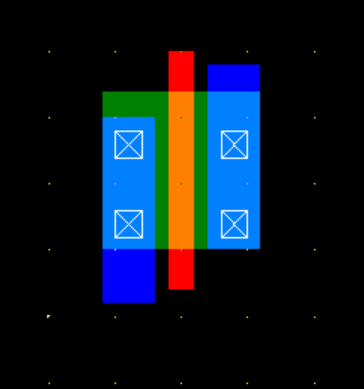
\includegraphics[scale=0.50]{./images/nmos_layout.PNG}
	\caption{NMOS Layout}
	\label{fig:nmos}
\end{figure}

\FloatBarrier

Figure (\ref{fig:nmos}) shows an NMOS transistor's layout. Figure (\ref{fig:l1_mos}) depicts the $I_{DS}$ versus $V_{DS}$ curve of the level 1 NMOS model.

\FloatBarrier

\begin{figure}[h!]
	\centering
	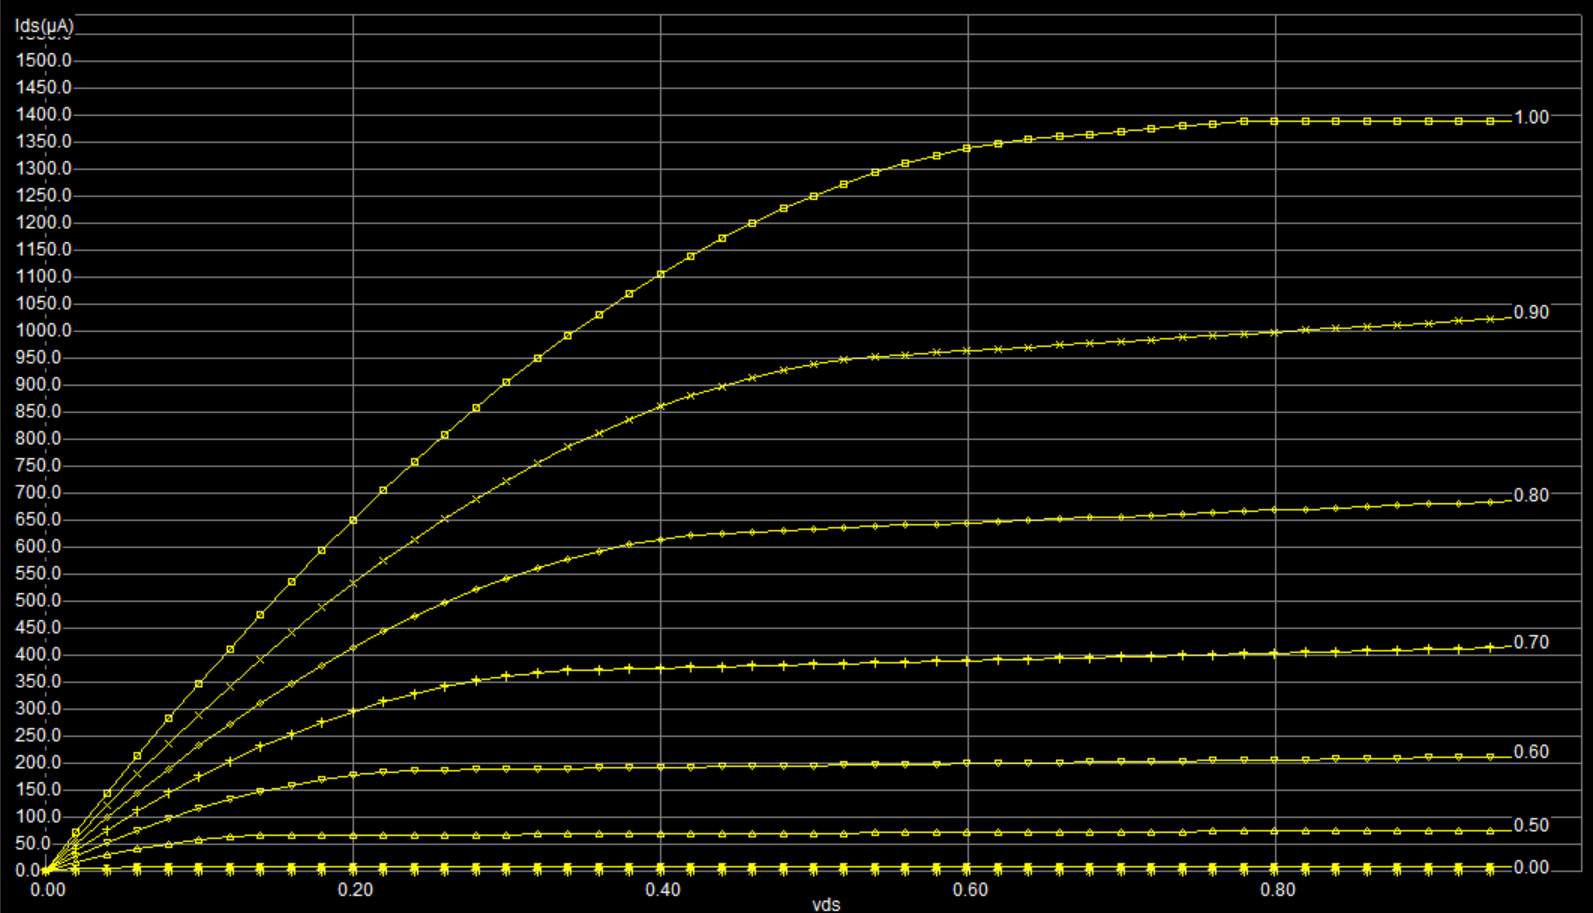
\includegraphics[scale=0.50]{./images/level1_id_vds_nmos.PNG}
	\caption{Level 1 NMOS Model}
	\label{fig:l1_mos}
\end{figure}

\FloatBarrier

The L1 NMOS model is a standard transistor model that accounts for some channel length modulation effects (very slight slope in the saturation graph).
When $V_{DS} = V_{GS} - V_{T}$, the current tapers off, and the MOSFET enters the saturation region.

\FloatBarrier

\begin{figure}[h!]
	\centering
	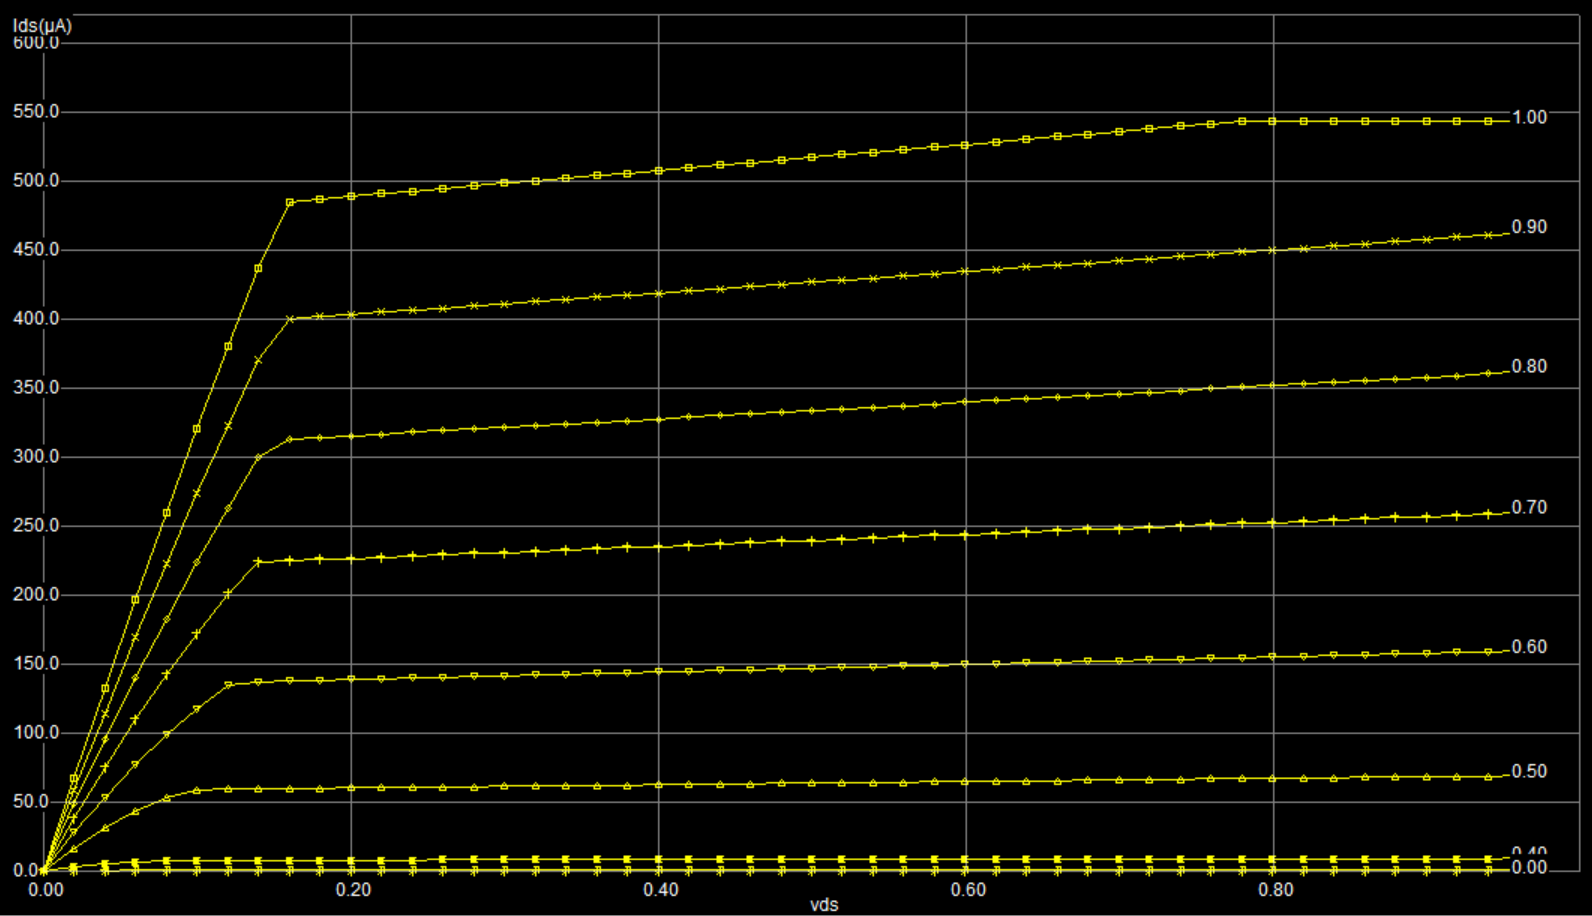
\includegraphics[scale=0.50]{./images/level3_id_vds_nmos.PNG}
	\caption{Level 3 NMOS Model}
	\label{fig:l3_mos}
\end{figure}

\FloatBarrier

L3 is an improvement that accounts for effects that cause the transistor to enter saturation at lower voltages.
This may be a short-channel effect in integrated circuits.
If the channel is sufficiently short, the depletion regions at the source and drains can extend into the channel.
As a result, the transistor may enter saturation at lower voltages since the depletion regions extend into the channel at higher drain voltages in saturation.
This is the cause of channel length modulation.

\FloatBarrier

\begin{figure}[h!]
	\centering
	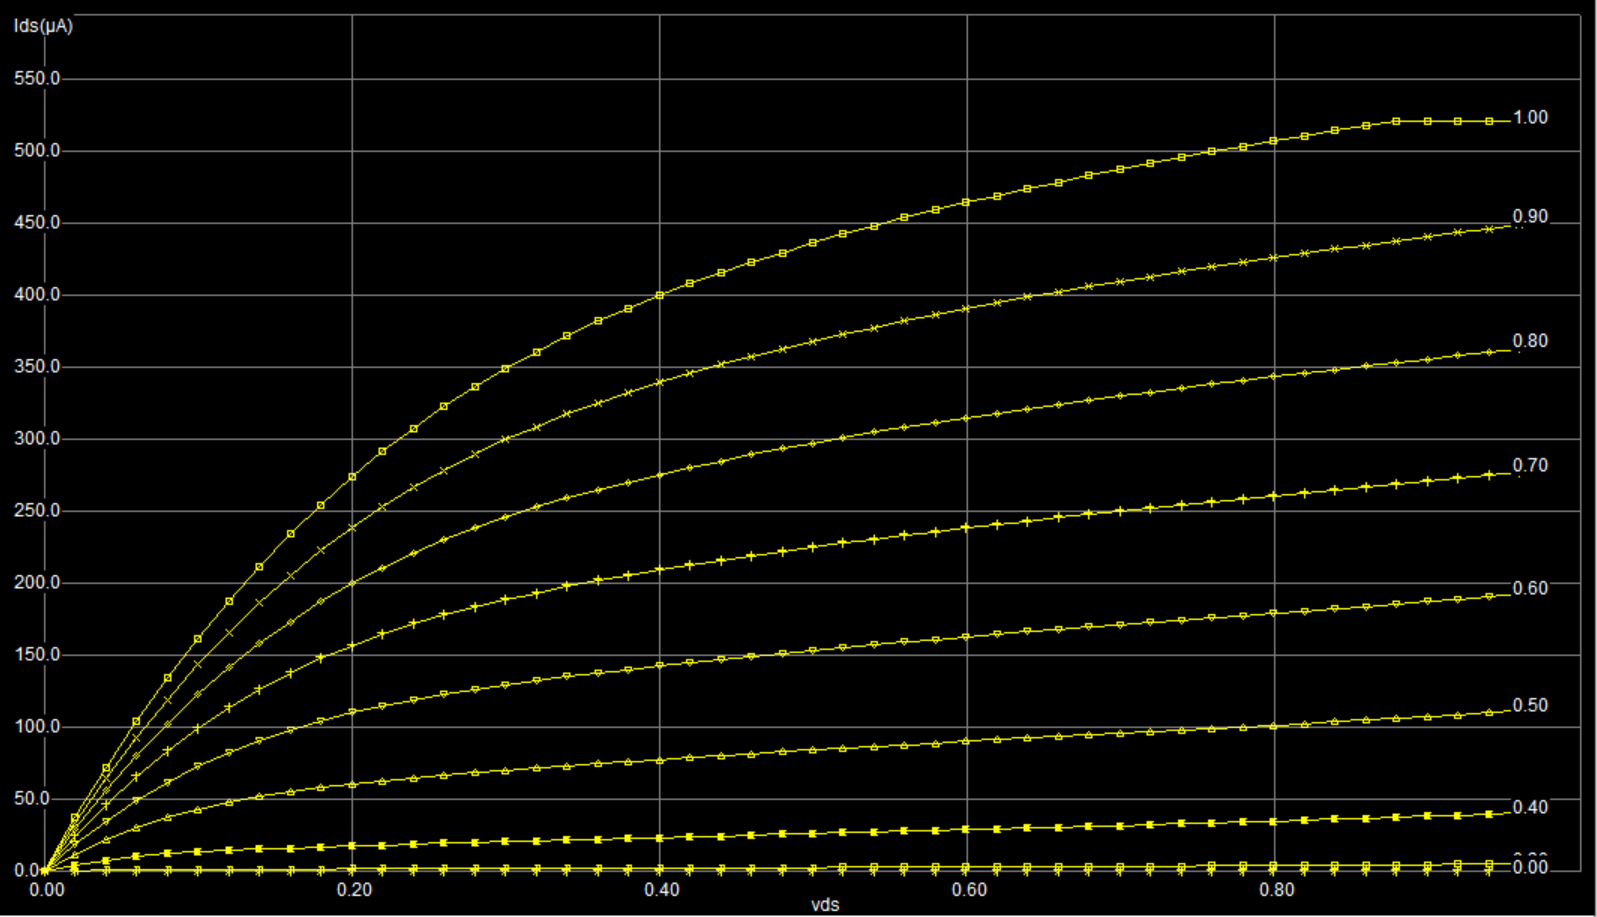
\includegraphics[scale=0.50]{./images/bsim4_id_vds_nmos.PNG}
	\caption{BSIM4 NMOS Model}
	\label{fig:bsim4_mos}
\end{figure}

\FloatBarrier

The BSIM4 model accounts for channel length modulation, which explains why the current increases linearly with $V_{DS}$ in saturation.
However, it is much more complicated in nature than the other two models in terms of its level of sophistication.
Level 3's triode region is quite linear. However, the model typically considered in lab uses polynomial growth that depends on at least $V_{DS}^2$ and possibly $V_{DS}^3$ with channel-length modulation.
The channel-length modulation effect in BSIM4 is a bit more pronounced than it is typically in the models used in the course.
From these plots, level 1 seems to be the closest to the currently used transistor model.
However, the $i_{D}$ vs $V_{GS}$ plots give a clearer view.

\FloatBarrier

\begin{figure}[h!]
	\centering
	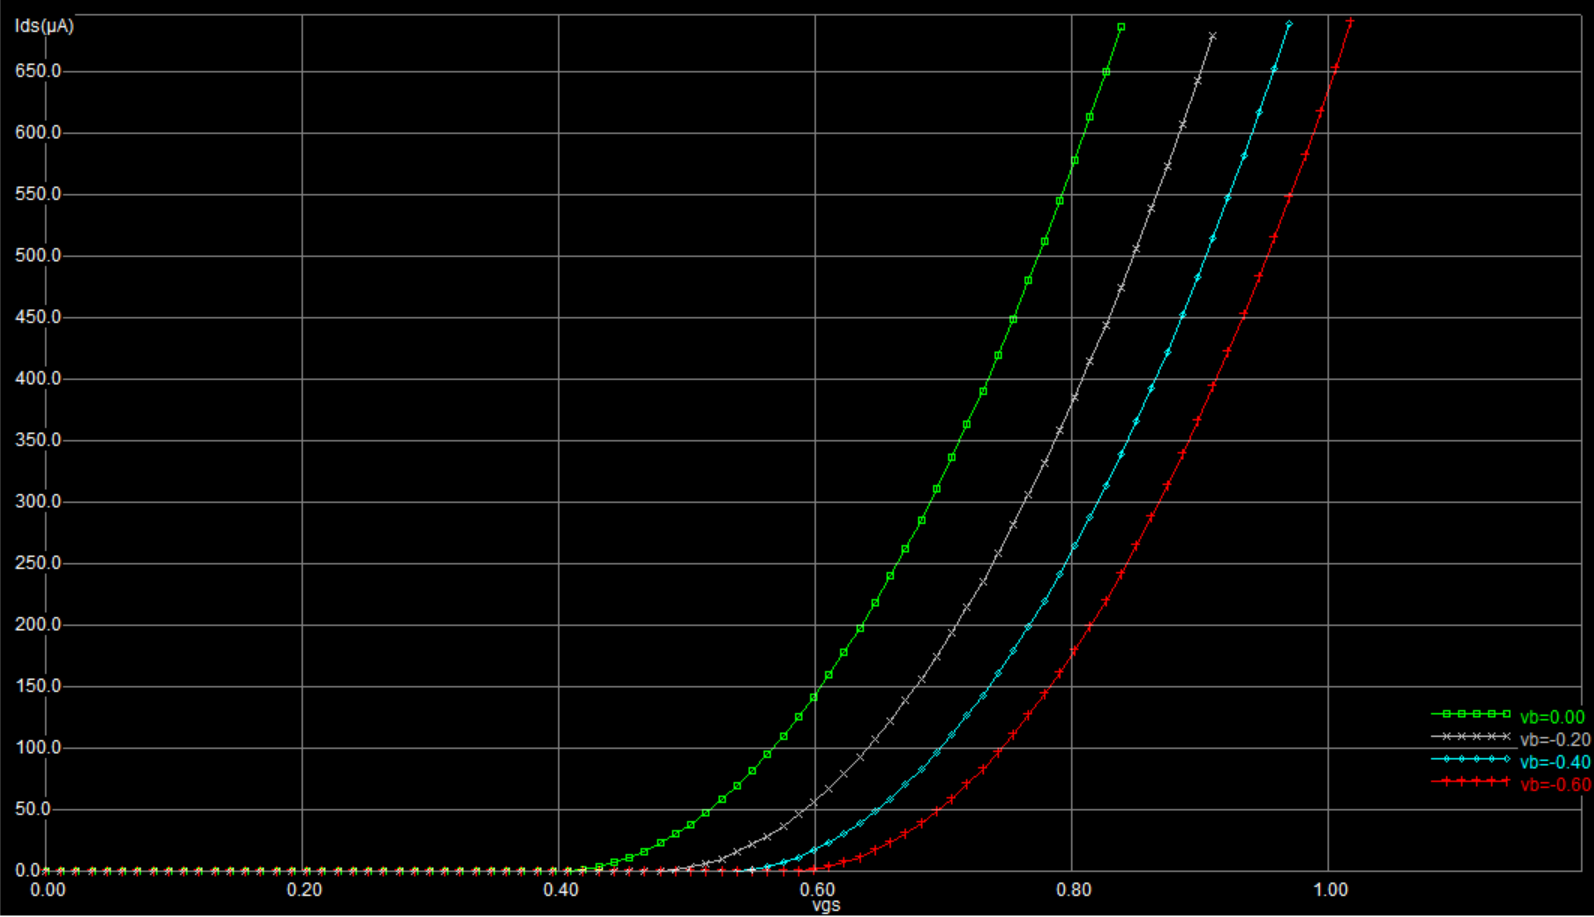
\includegraphics[scale=0.50]{./images/id_vgs_level1.PNG}
	\caption{Level 1 $i_{D}$ versus $V_{GS}$}
	\label{fig:id_vgs_level1}
\end{figure}

\FloatBarrier

\FloatBarrier

\begin{figure}[h!]
	\centering
	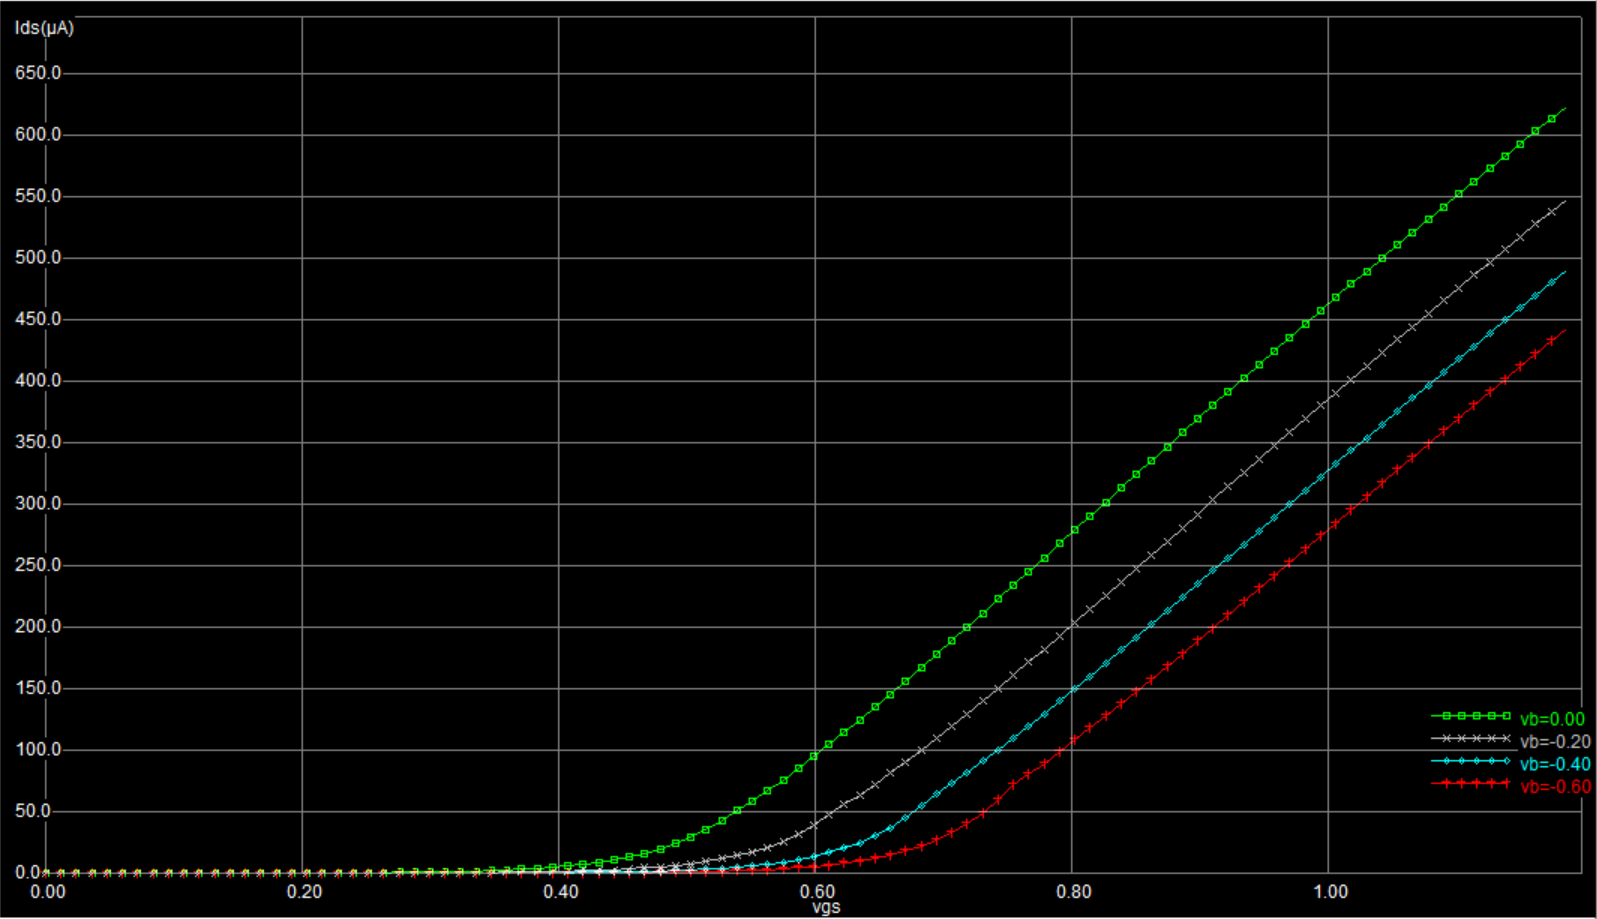
\includegraphics[scale=0.50]{./images/id_vgs_level3.PNG}
	\caption{Level 3 $i_{D}$ versus $V_{GS}$}
	\label{fig:id_vgs_level3}
\end{figure}

\FloatBarrier

\FloatBarrier

\begin{figure}[h!]
	\centering
	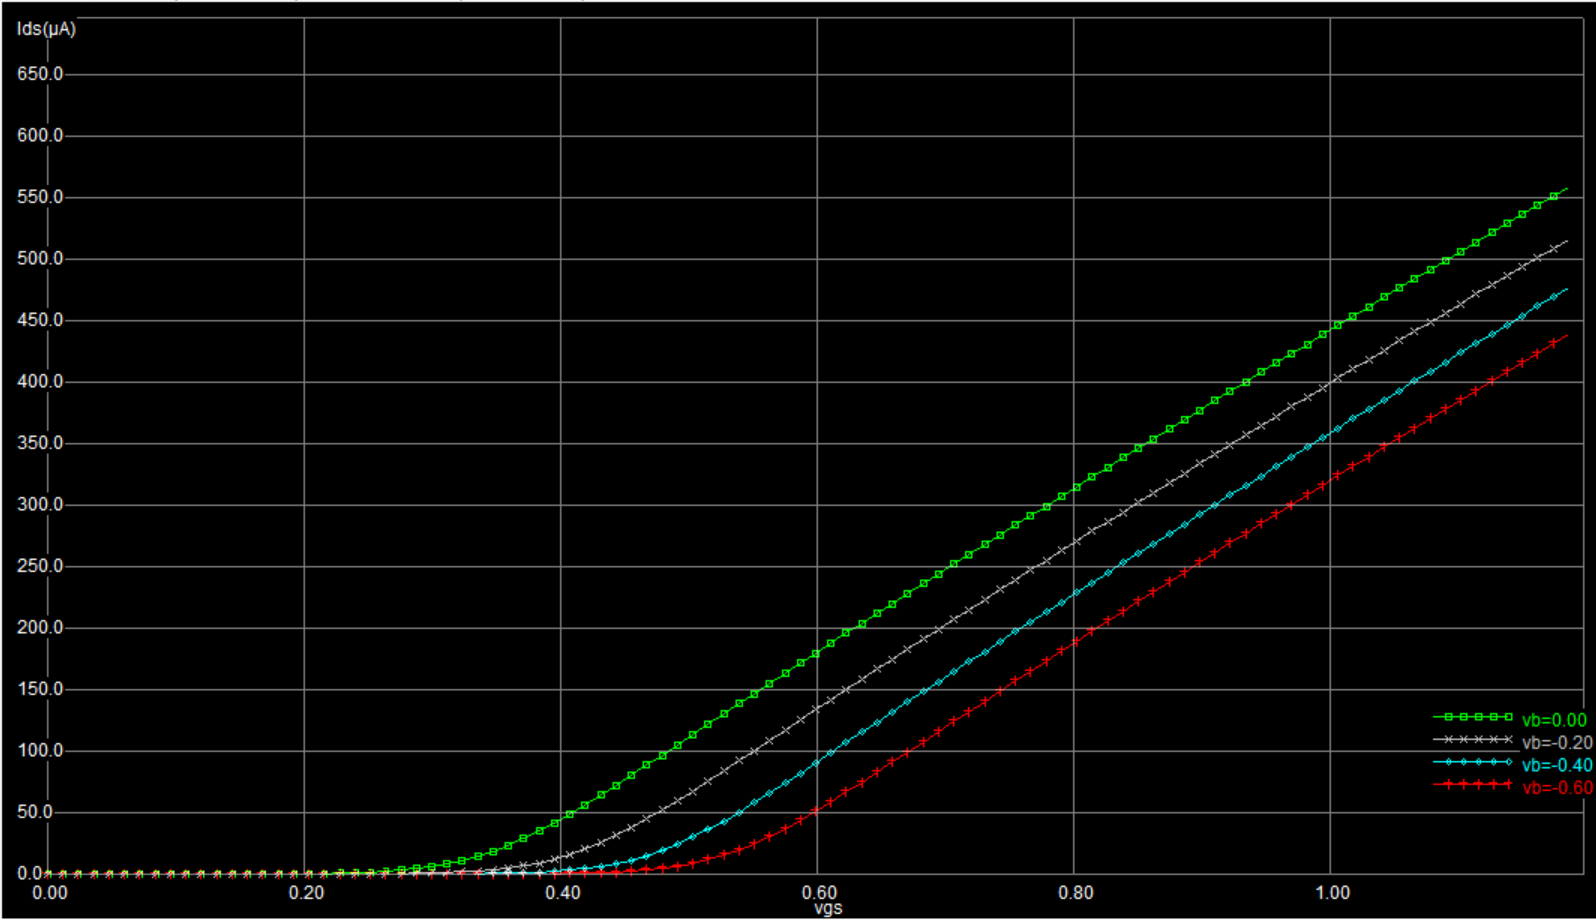
\includegraphics[scale=0.50]{./images/id_vgs_bsim4.PNG}
	\caption{BSIM4 $i_{D}$ versus $V_{GS}$}
	\label{fig:id_vgs_bsim4}
\end{figure}

\FloatBarrier

The level 1 model follows the quadratic relationship expected for the plot, whereas the other plots are more linear.
Therefore, the level 1 MOSFET model is closest to the one typically used in the course.

The body effect in a MOSFET occurs when the body is not grounded.
Typically, the NMOS body is set to the lowest voltage in the circuit.
However, if the body's voltage is decreased, it becomes harder to attract electrons to the body because the voltage is lower.
Therefore, the threshold voltage increases as the body voltage is decreased because it now requires a higher gate voltage to attract the electrons to form the channel.
This is evident from the transistor models.

\FloatBarrier

\begin{figure}[h!]
	\centering
	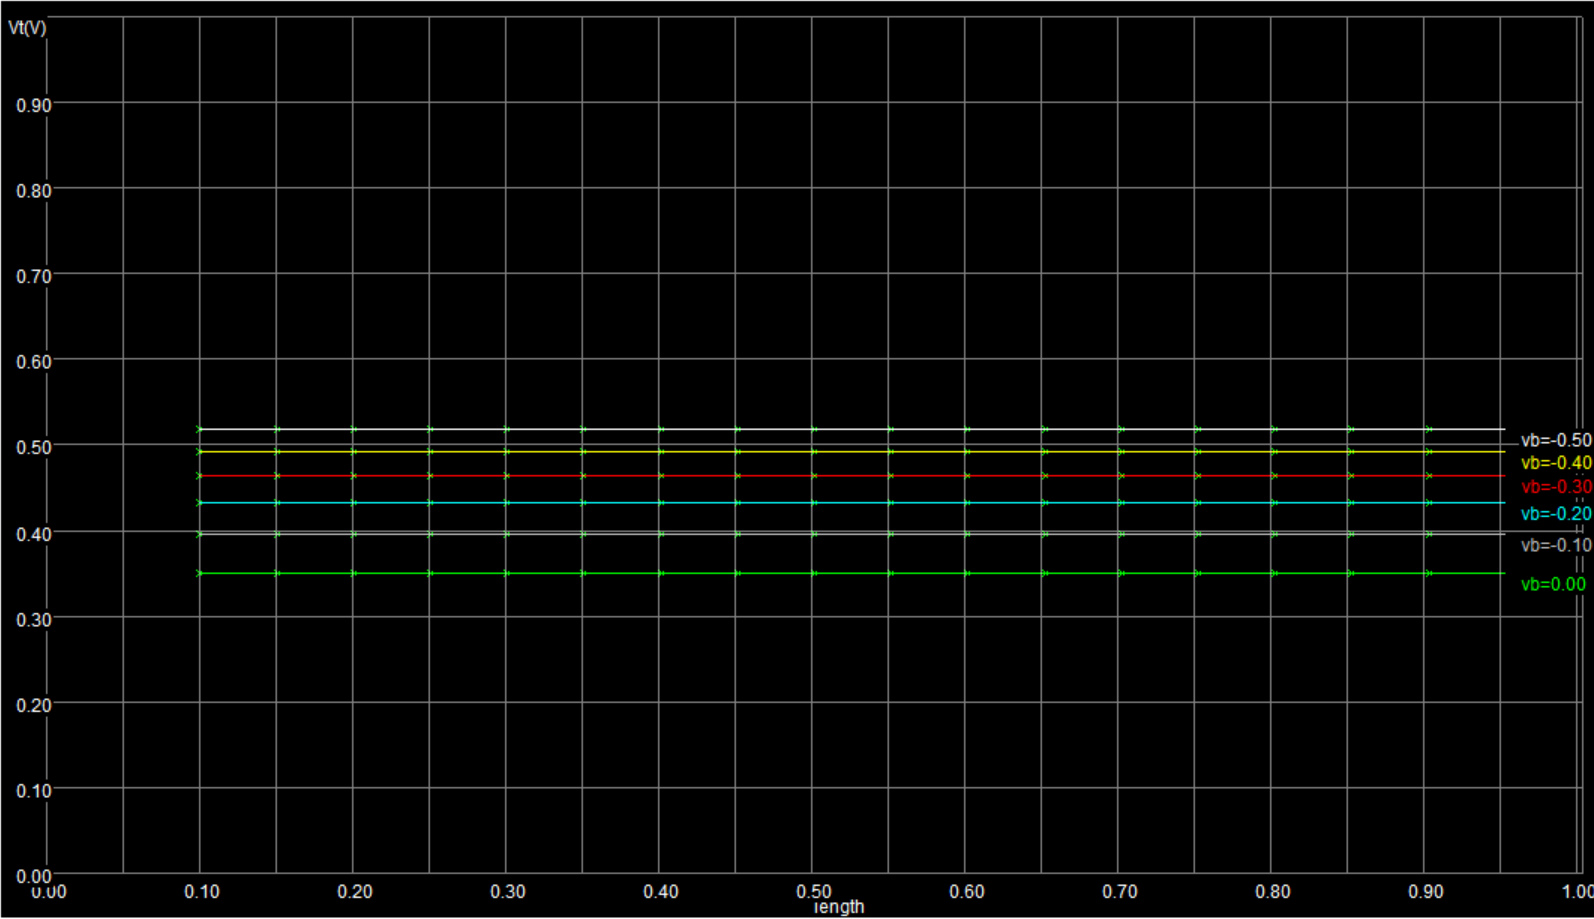
\includegraphics[scale=0.50]{./images/level1_body_effect_nmos.PNG}
	\caption{L1 NMOS Body Effect}
	\label{fig:l1_bodyeffect}
\end{figure}

\FloatBarrier

\FloatBarrier

\begin{figure}[h!]
	\centering
	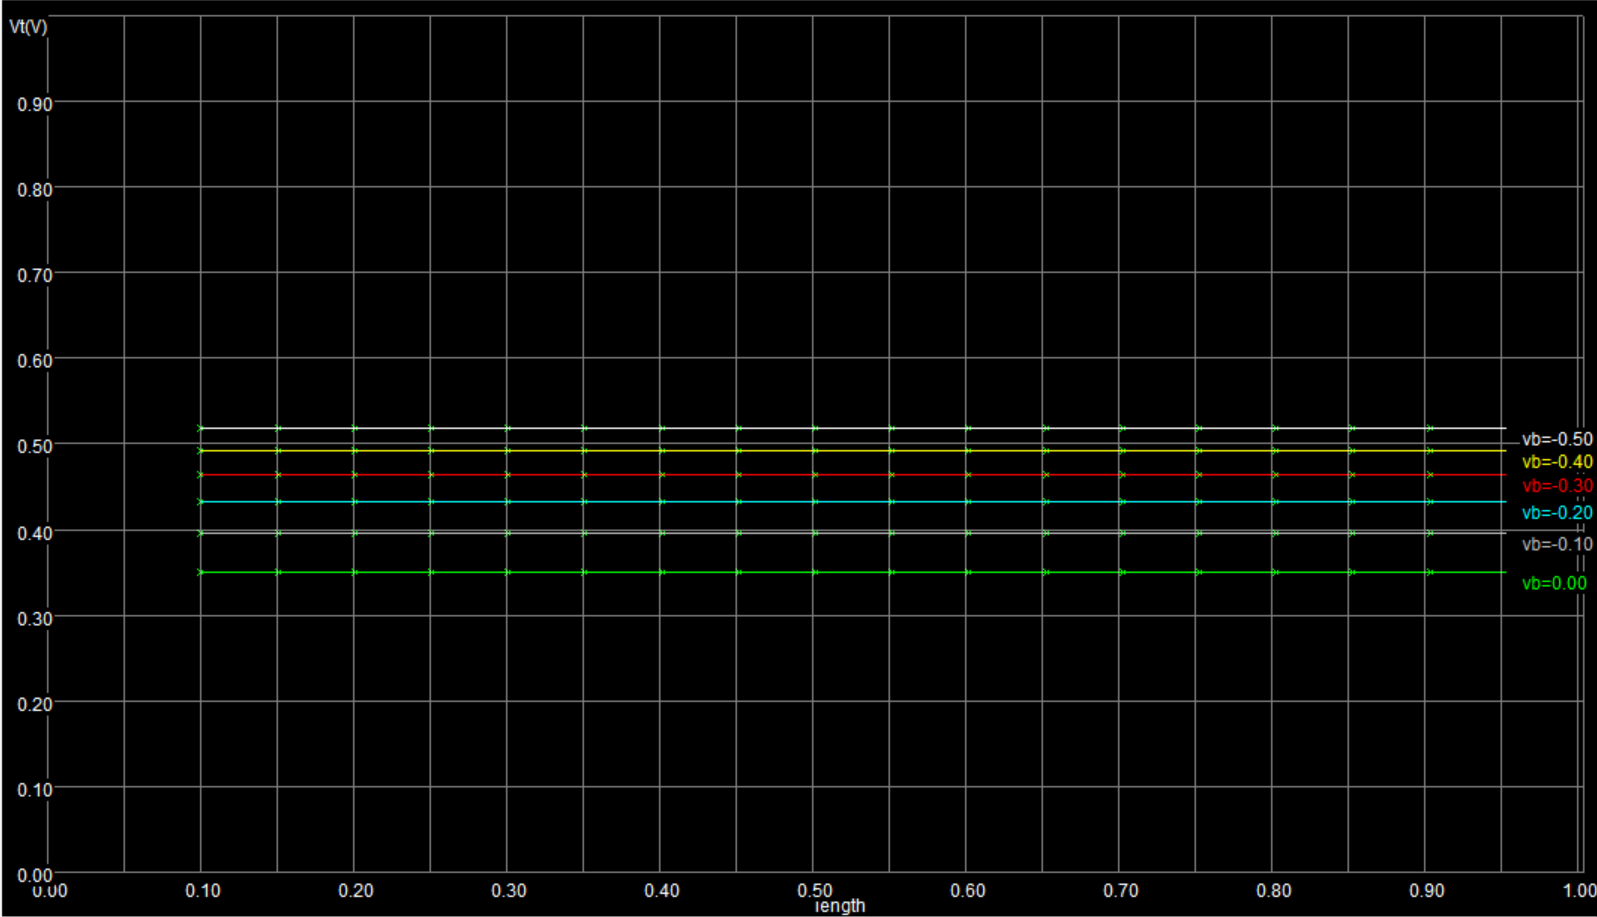
\includegraphics[scale=0.50]{./images/level3_body_effect_nmos.PNG}
	\caption{L3 NMOS Body Effect}
	\label{fig:l3_bodyeffect}
\end{figure}

\FloatBarrier

The body effect observed in figures (\ref{fig:l1_bodyeffect}) and (\ref{fig:l3_bodyeffect}) is essentially the same.
Decreasing the body voltage increases the threshold voltage.
If the threshold voltage increases, the overdrive voltage drops, and the current therefore decreases.
So, decreasing the body voltage decreases the current.
In neither of these models does the body effect depend on the channel length.

\FloatBarrier

\begin{figure}[h!]
	\centering
	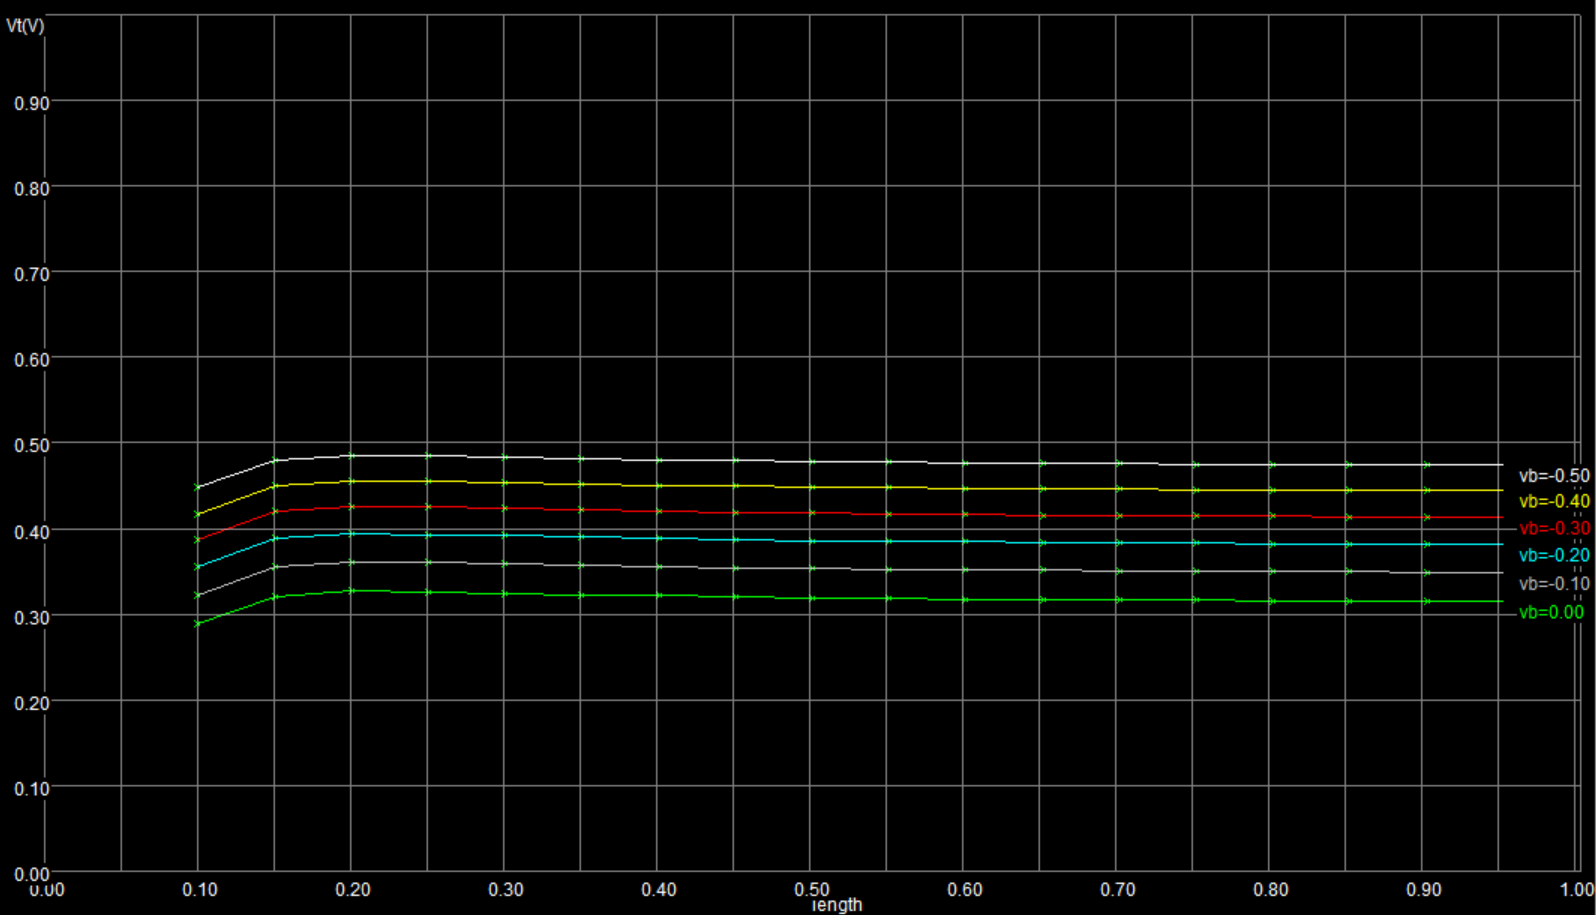
\includegraphics[scale=0.50]{./images/bsim4_body_effect_nmos.PNG}
	\caption{BSIM4 NMOS Body Effect}
	\label{fig:bsim4_bodyeffect}
\end{figure}

\FloatBarrier

The BSIM4 model accounts for effects that occur in submicron processes when the channel length becomes very short.
The threshold voltage drops when the channel length is very short.
This might be because the depletion layers from the source and the drain help facilitate the motion of charges in the channel, meaning fewer charges and therefore a lower gate voltage is required to sustain an adequate current.
The SPICE model typically used in lab does not seem to contain information on such short-channel effects, but does contain information about junction capacitances with the body, meaning that it probably accounts for some body effects.
Again, level 1 seems closest to the SPICE model provided, whereas level 3 and especially BSIM4 are much more sophisticated. \\

If the oxide layer thickness is increased, the MOS capacitor's capacitance is decreased.
Thus, for the same applied gate voltage, less charge accumulates in the channel.
Therefore, ceteris paribus, the current should decrease if the oxide layer thickness is increased. \\

The MOSFET model used in the course is somewhat accurate and captures some nonidealities in a true integrated circuit MOSFET, such as channel-length modulation.
However, at deeper submicron processes, other short-channel effects come to play. These affect threshold voltages as well as the current.
So, the MOSFET model can possibly be used for larger transistor processes, but more sophisticated models such as Level 3 or even BSIM4 are required for a modern integrated circuit design.

\FloatBarrier

\begin{figure}[h!]
	\centering
	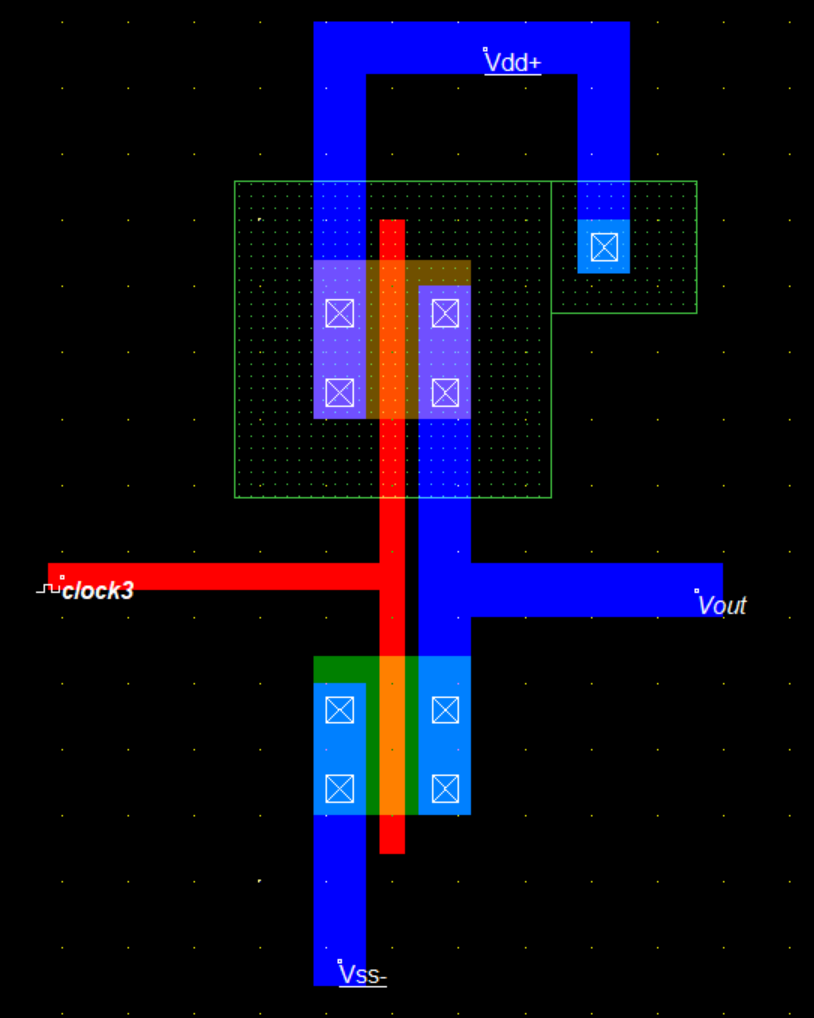
\includegraphics[scale=0.75]{./images/inverter_06nmos06pmos.PNG}
	\caption{Layout of CMOS Inverter - 0.6\si{\micro\meter} Width for NMOS and PMOS}
	\label{fig:inverter_layout}
\end{figure}

\FloatBarrier

The CMOS inverter can be implemented in a true integrated circuit process, depicted in figure (\ref{fig:inverter_layout}).
The design depicted passes the design rule check.

\FloatBarrier

\begin{figure}[h!]
	\centering
	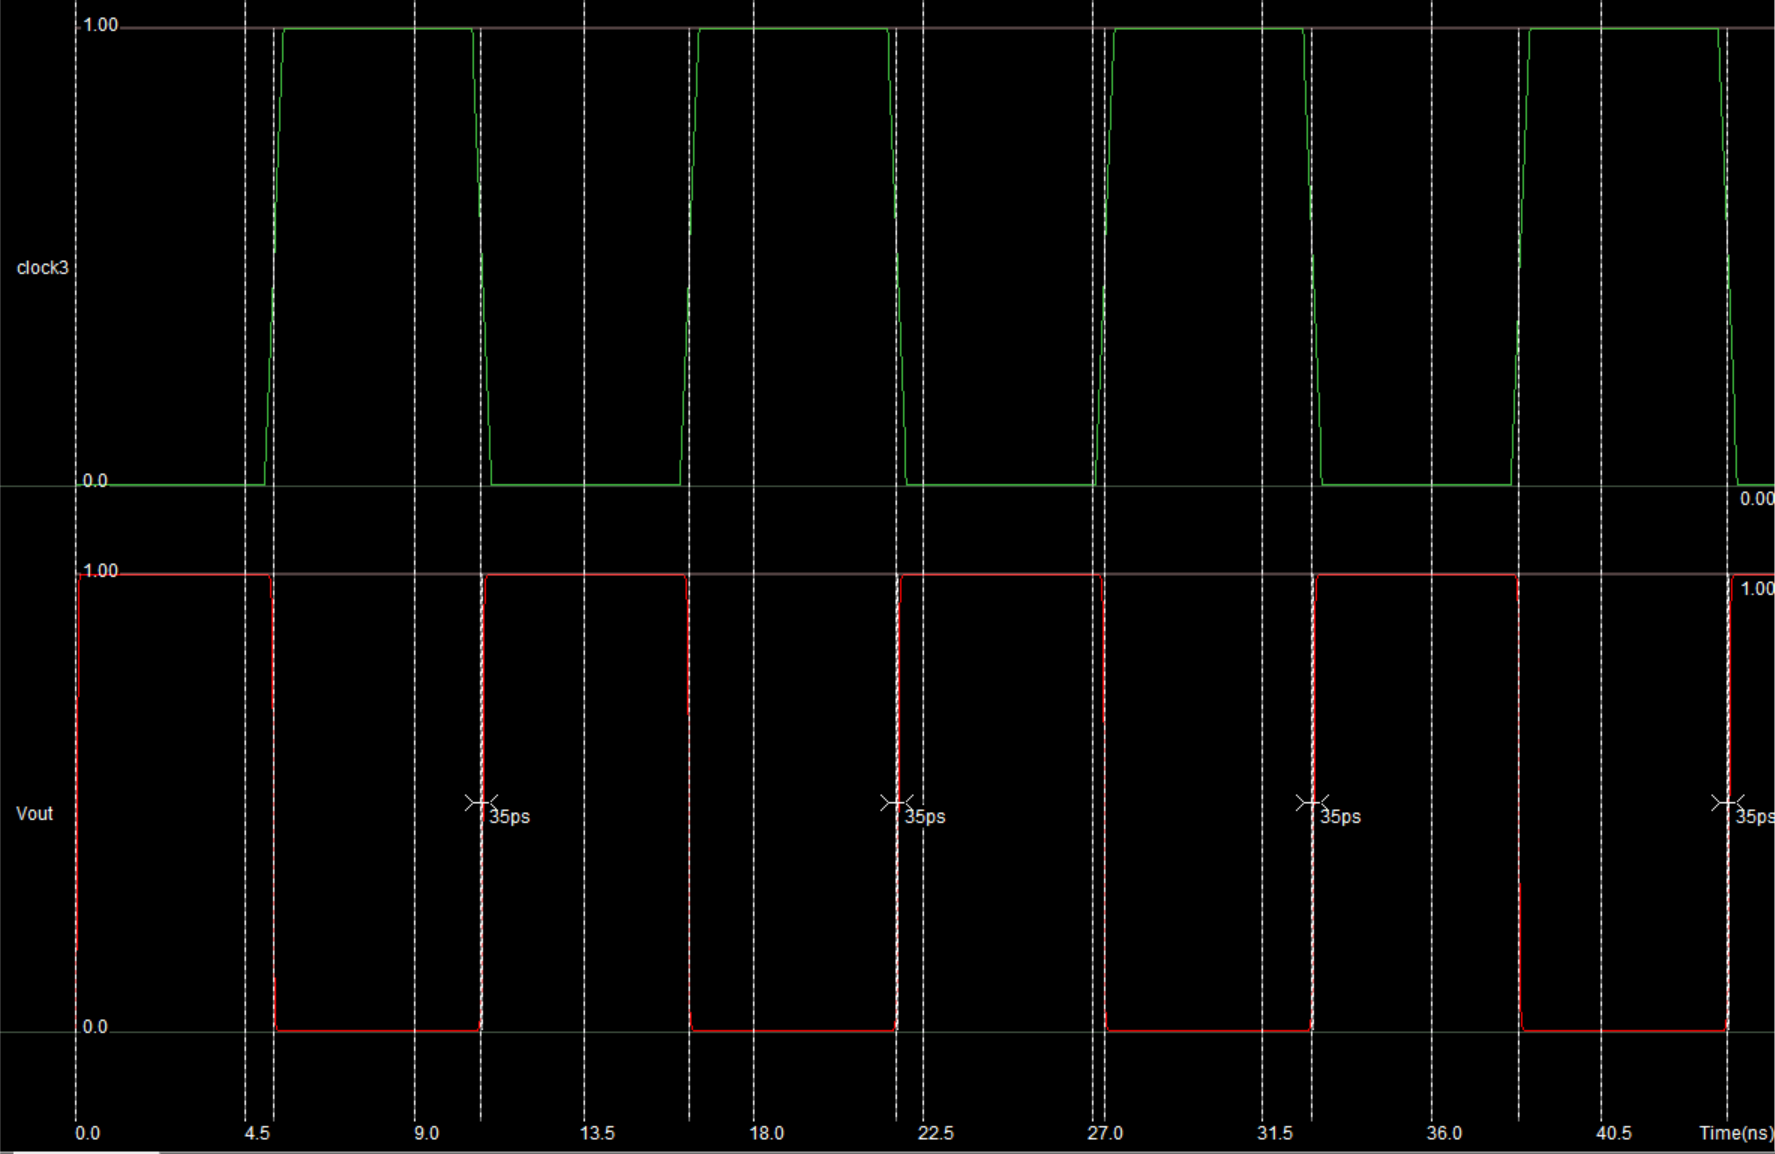
\includegraphics[scale=0.50]{./images/inverter_transient_06nmos_06pmos.PNG}
	\caption{CMOS Inverter Layout Transient Response - 0.6\si{\micro\meter} Width for NMOS and PMOS}
	\label{fig:cmos_layout_transient}
\end{figure}

\FloatBarrier

\FloatBarrier

\begin{figure}[h!]
	\centering
	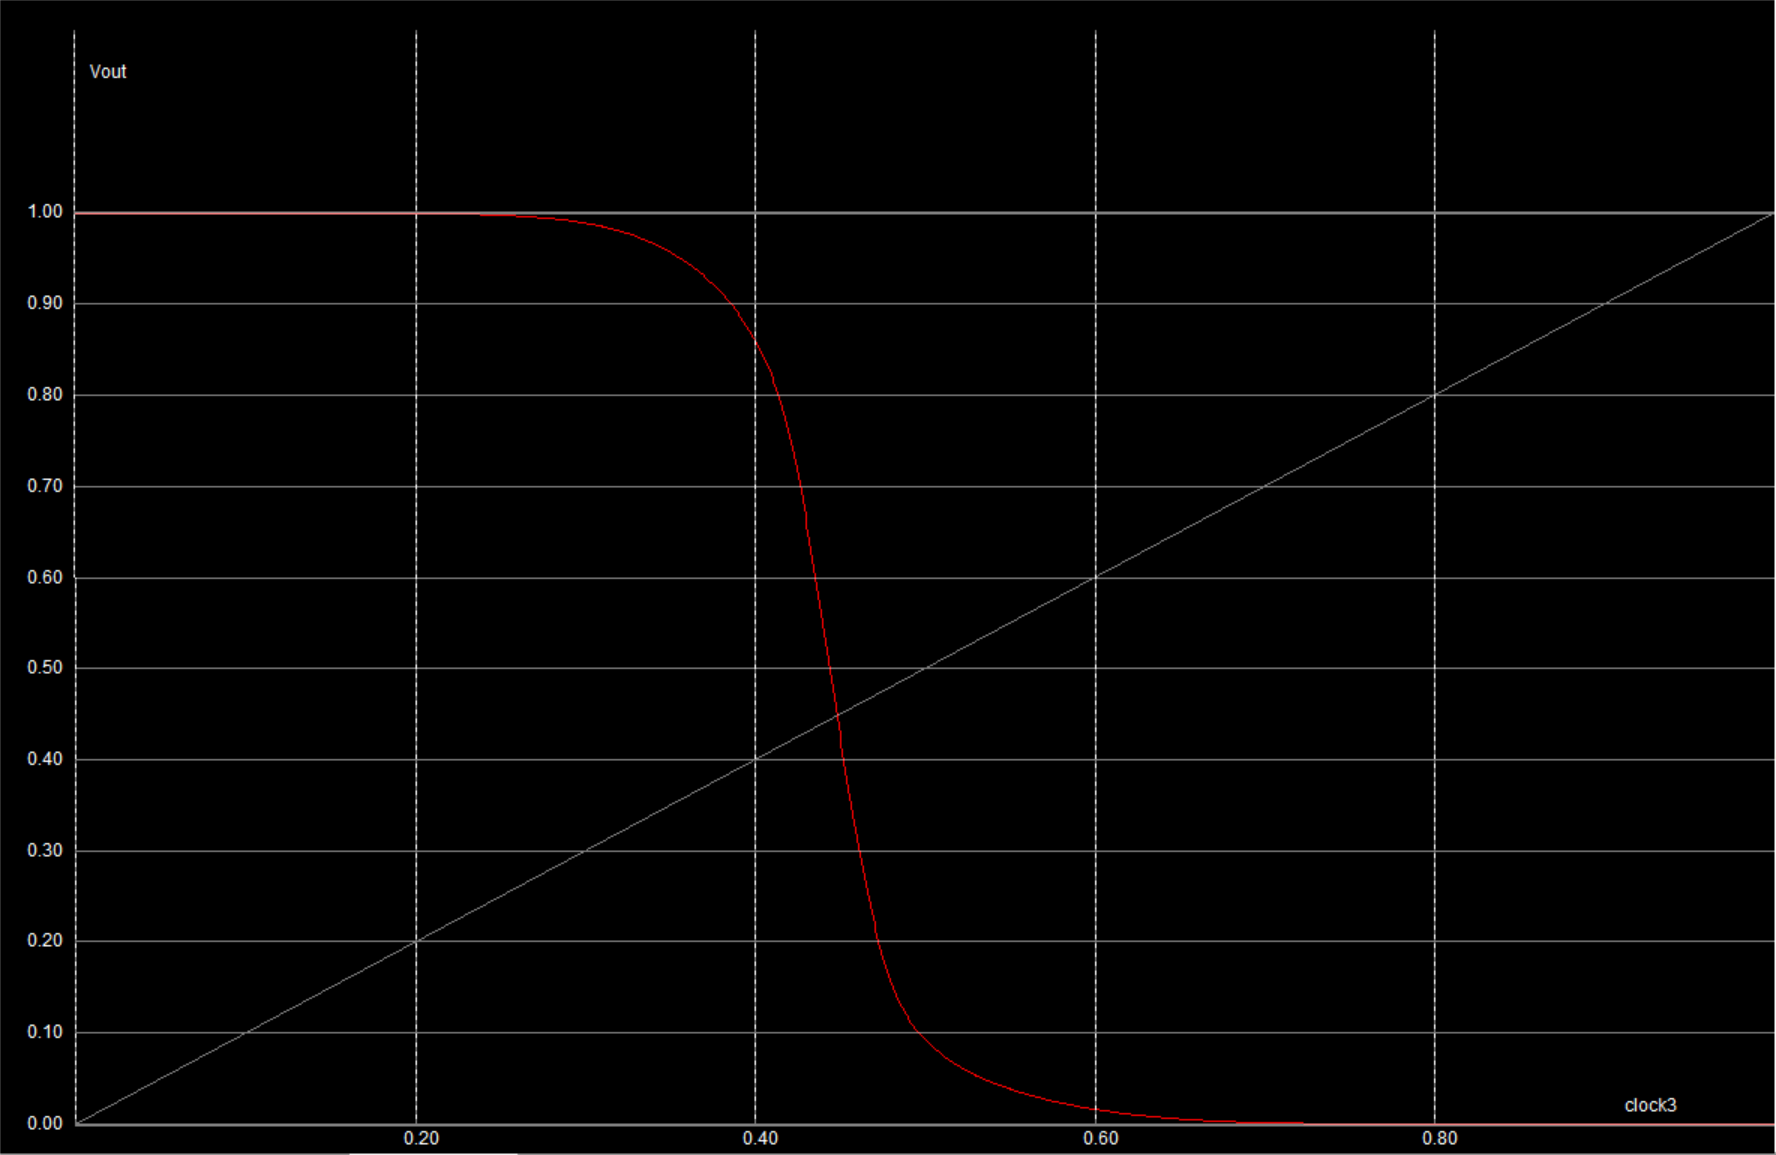
\includegraphics[scale=0.50]{./images/inverter_vtc_06nmos_06pmos.PNG}
	\caption{CMOS Inverter Layout Voltage Transfer Characteristic (VTC) - 0.6\si{\micro\meter} Width for NMOS and PMOS}
	\label{fig:cmos_layout_vtc}
\end{figure}

\FloatBarrier

Figure (\ref{fig:cmos_layout_transient}) presents the transient response of the inverter.
Figure (\ref{fig:cmos_layout_vtc}) depicts the voltage transfer characteristic.
The nature of the results is similar to those presented in SPICE simulations earlier.
Two inverters are then cascaded to observe the loading effects and changes in propagation delay.

\FloatBarrier

\begin{figure}[h!]
	\centering
	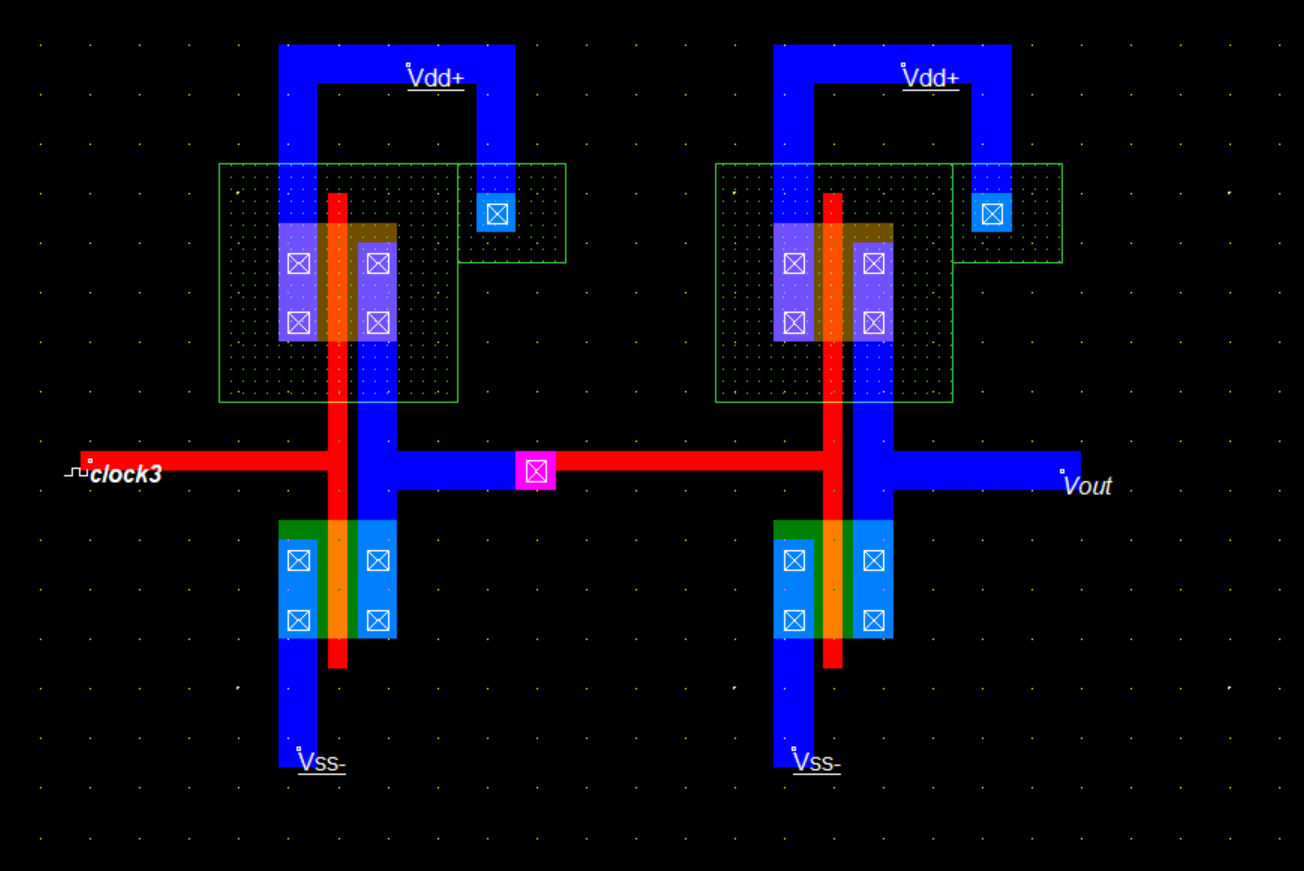
\includegraphics[scale=0.75]{./images/cascaded_inverter_06nmos06pmos.PNG}
	\caption{Cascaded Inverter Layout - 0.6\si{\micro\meter} Width for NMOS and PMOS}
	\label{fig:cascaded_inverter_06nmos06pmos}
\end{figure}

\FloatBarrier

\FloatBarrier

\begin{figure}[h!]
	\centering
	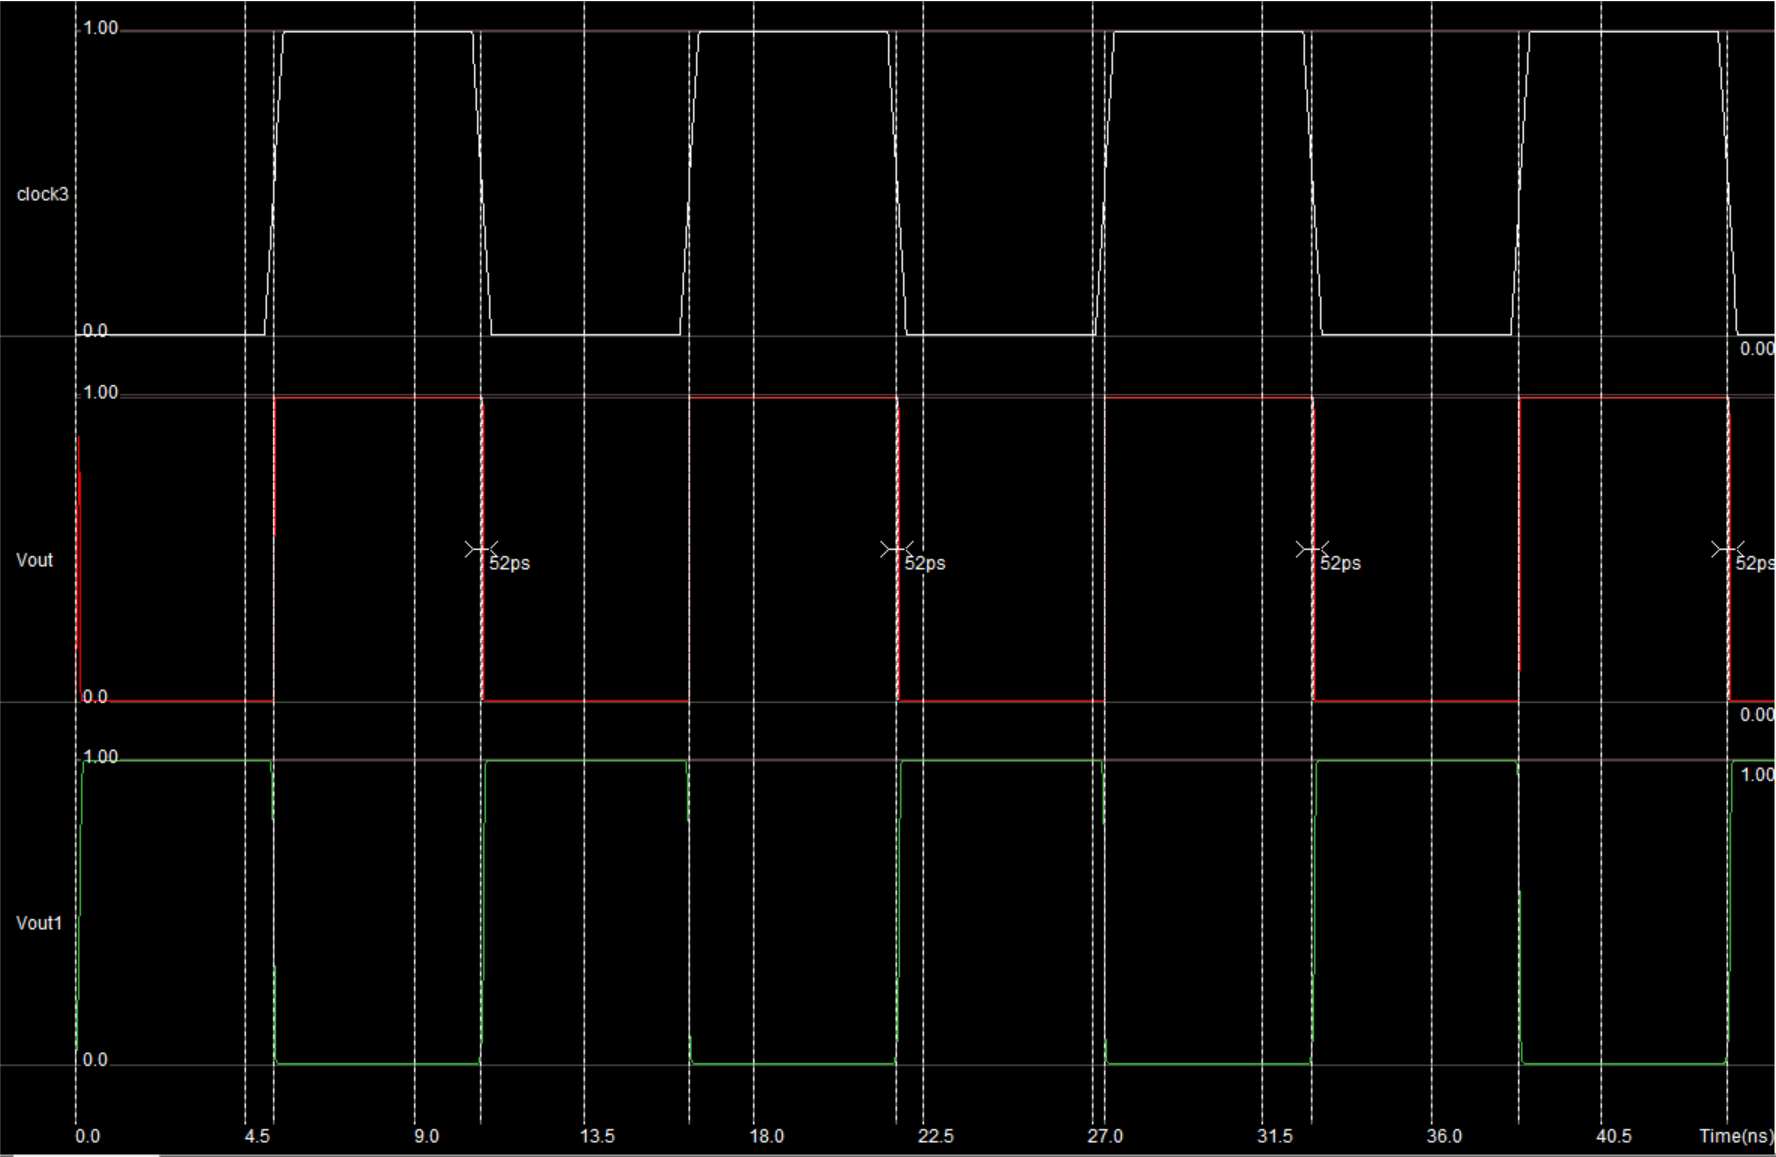
\includegraphics[scale=0.50]{./images/cascaded_inverter_transient_06nmos06pmos.PNG}
	\caption{Cascaded Inverter Transient - 0.6\si{\micro\meter} Width for NMOS and PMOS}
	\label{fig:cascaded_inverter_transient_06nmos06pmos}
\end{figure}

\FloatBarrier

The results below are obtained when the NMOS width is kept the same, but the PMOS width is increased to 1.5\si{\micro\meter}.

\FloatBarrier

\begin{figure}[h!]
	\centering
	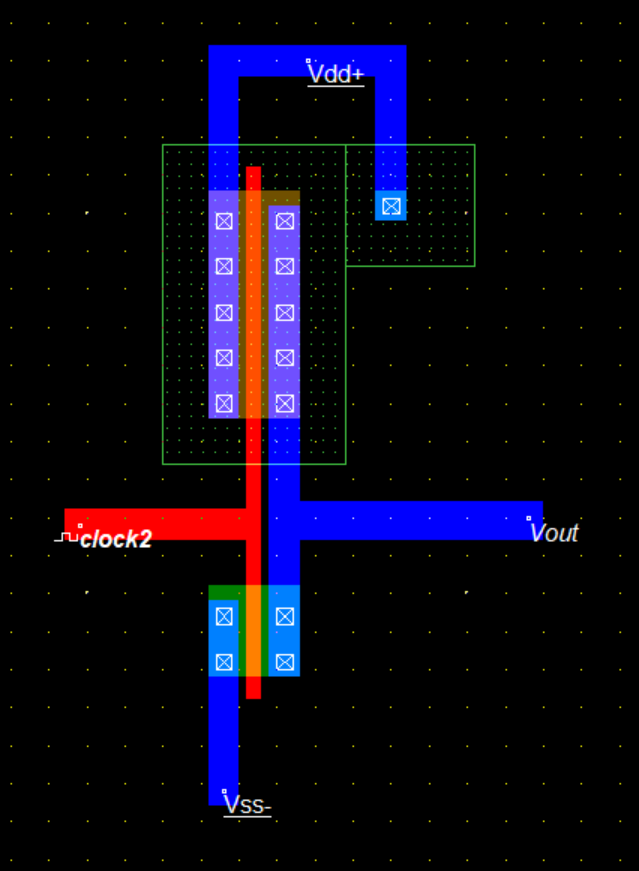
\includegraphics[scale=0.75]{./images/inverter_06nmos15pmos.PNG}
	\caption{Layout of CMOS Inverter - 0.6\si{\micro\meter} Width for NMOS, 1.5 \si{\micro\meter} Width for PMOS}
	\label{fig:inverter_06nmos15pmos}
\end{figure}

\FloatBarrier

\FloatBarrier

\begin{figure}[h!]
	\centering
	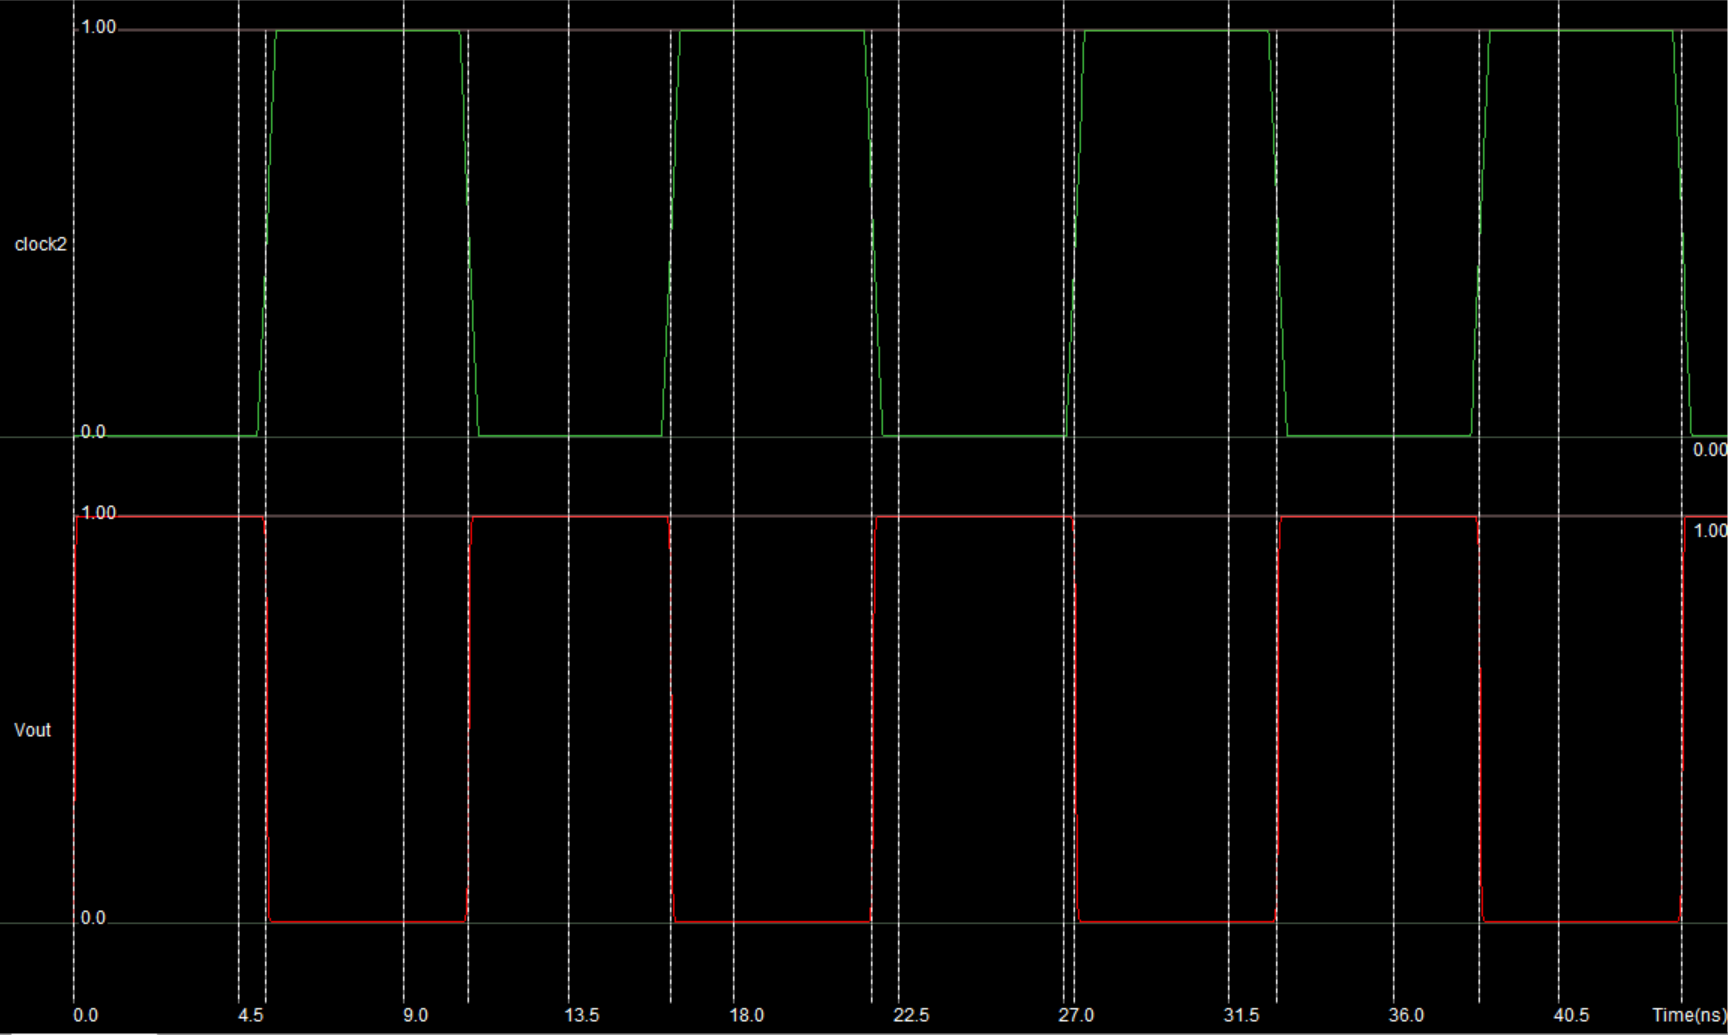
\includegraphics[scale=0.50]{./images/inverter_transient_06nmos_15pmos.PNG}
	\caption{CMOS Inverter Layout Transient Response - 0.6\si{\micro\meter} Width for NMOS, 1.5 \si{\micro\meter} Width for PMOS}
	\label{fig:inverter_transient_06nmos_15pmos}
\end{figure}

\FloatBarrier

\FloatBarrier

\begin{figure}[h!]
	\centering
	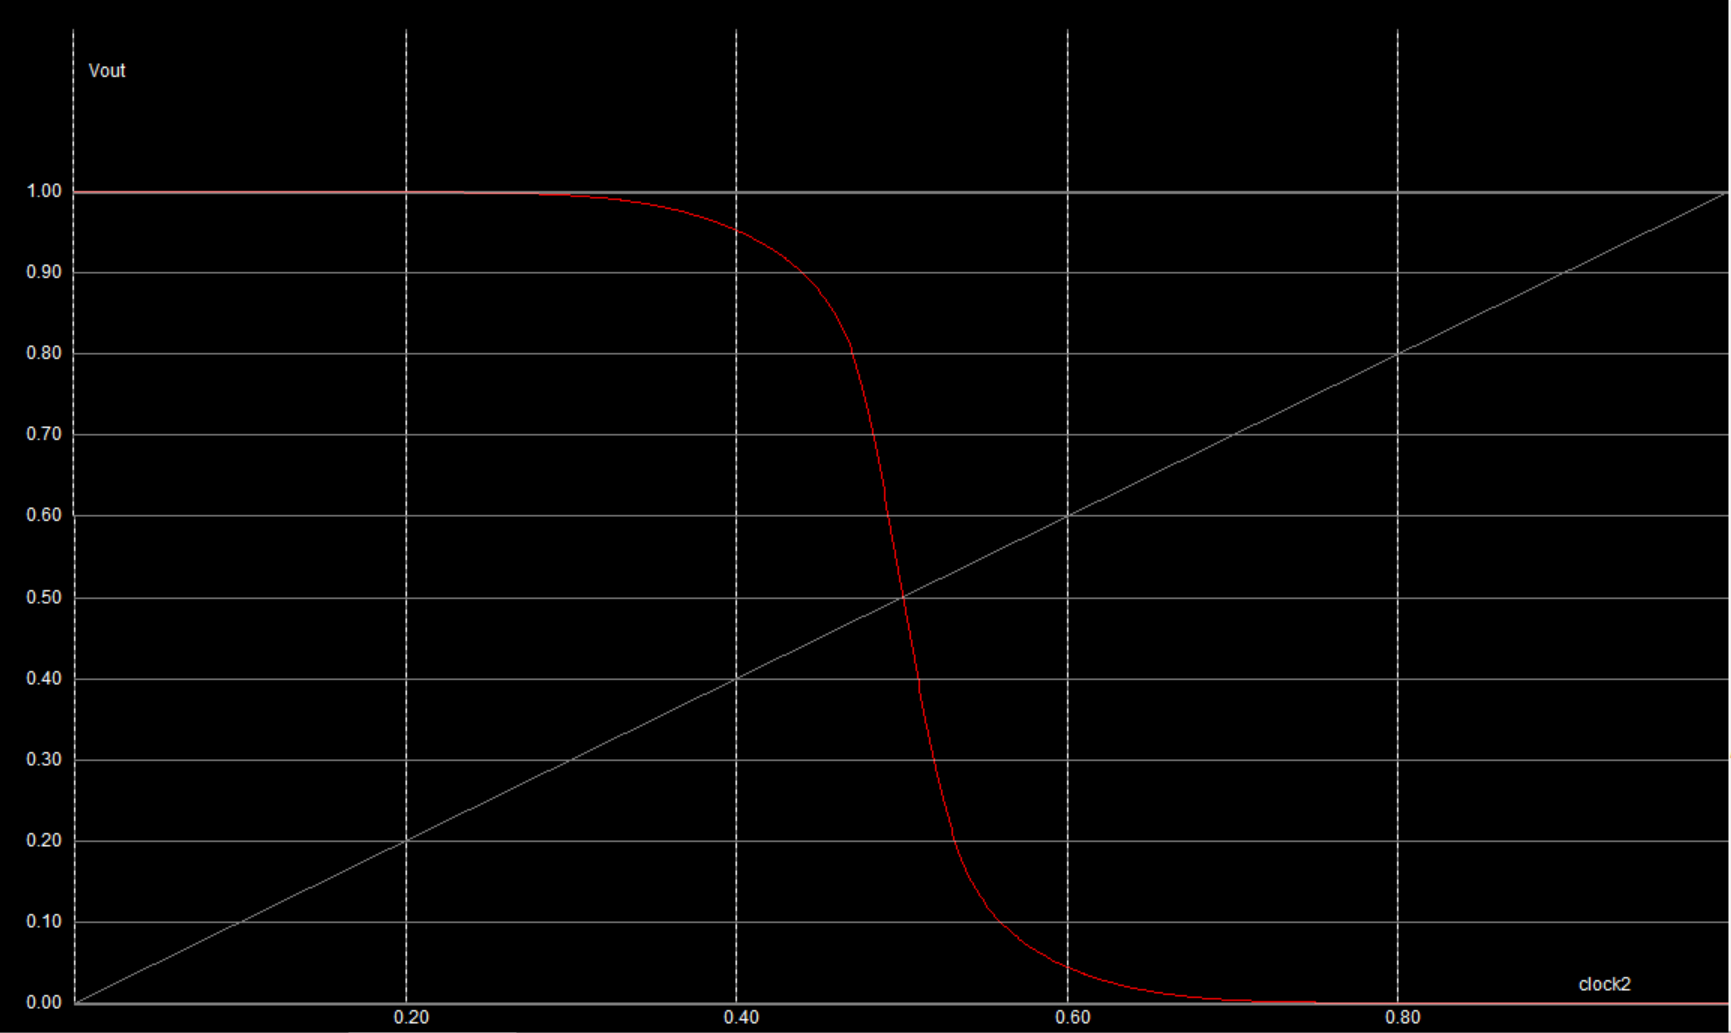
\includegraphics[scale=0.50]{./images/inverter_vtc_06nmos_15pmos.PNG}
	\caption{CMOS Inverter Layout Voltage Transfer Characteristic (VTC) - 0.6\si{\micro\meter} Width for NMOS, 1.5 \si{\micro\meter} Width for PMOS}
	\label{fig:inverter_vtc_06nmos_15pmos}
\end{figure}

\FloatBarrier

\FloatBarrier

\begin{figure}[h!]
	\centering
	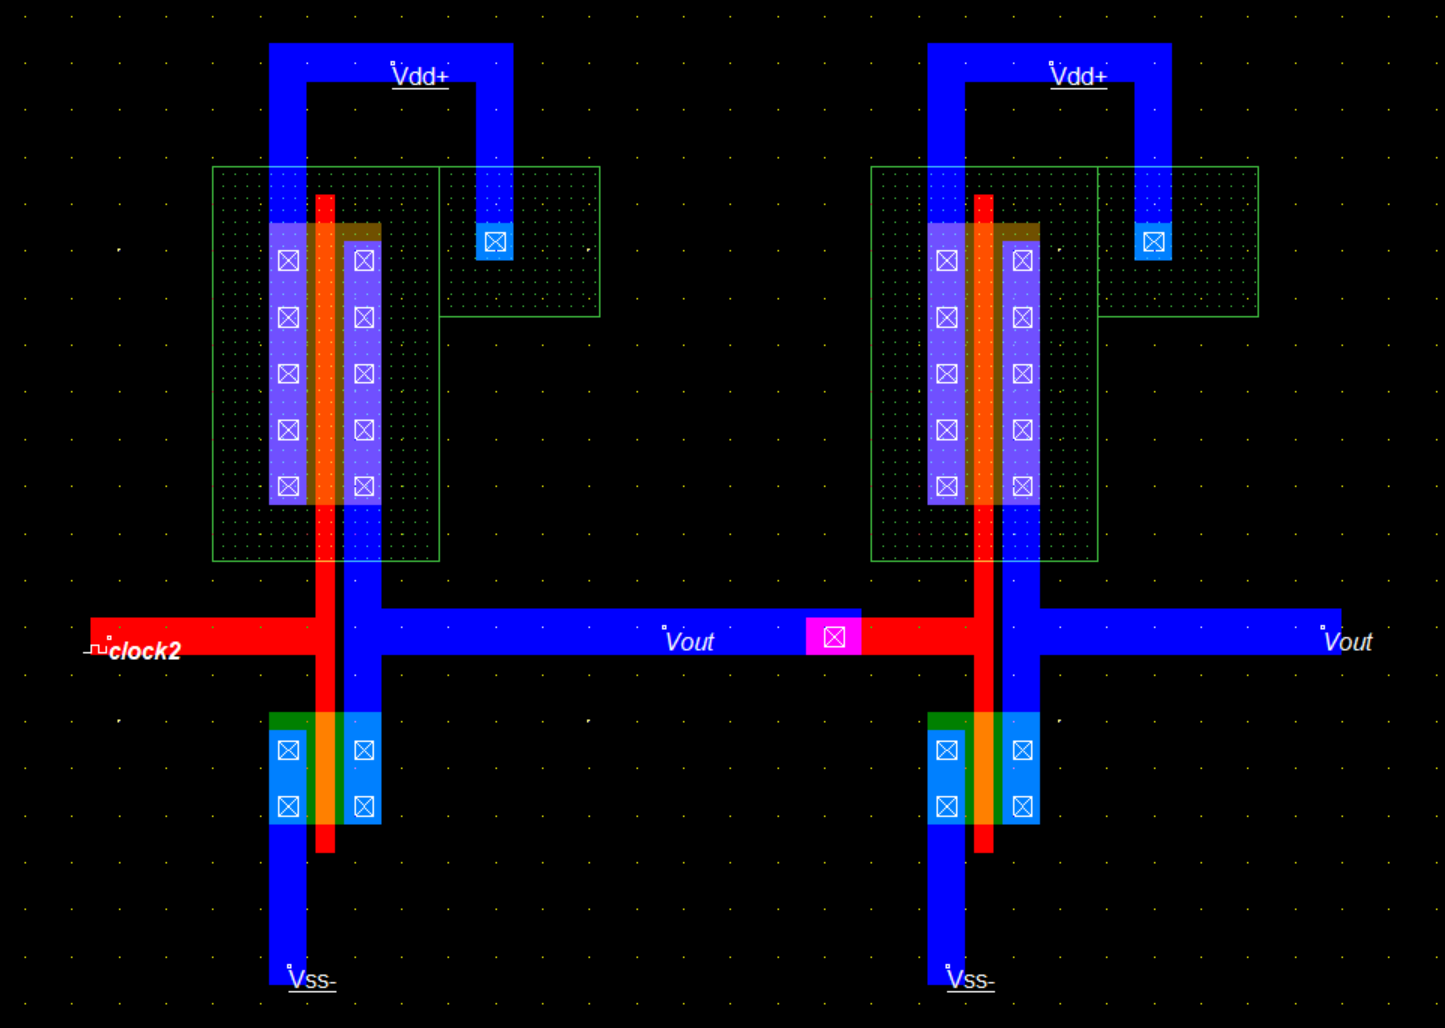
\includegraphics[scale=0.50]{./images/cascaded_inverter_06nmos15pmos.PNG}
	\caption{Cascaded Inverter Layout - 0.6\si{\micro\meter} Width for NMOS, 1.5 \si{\micro\meter} Width for PMOS}
	\label{fig:cascaded_inverter_06nmos15pmos}
\end{figure}

\FloatBarrier

\FloatBarrier

\begin{figure}[h!]
	\centering
	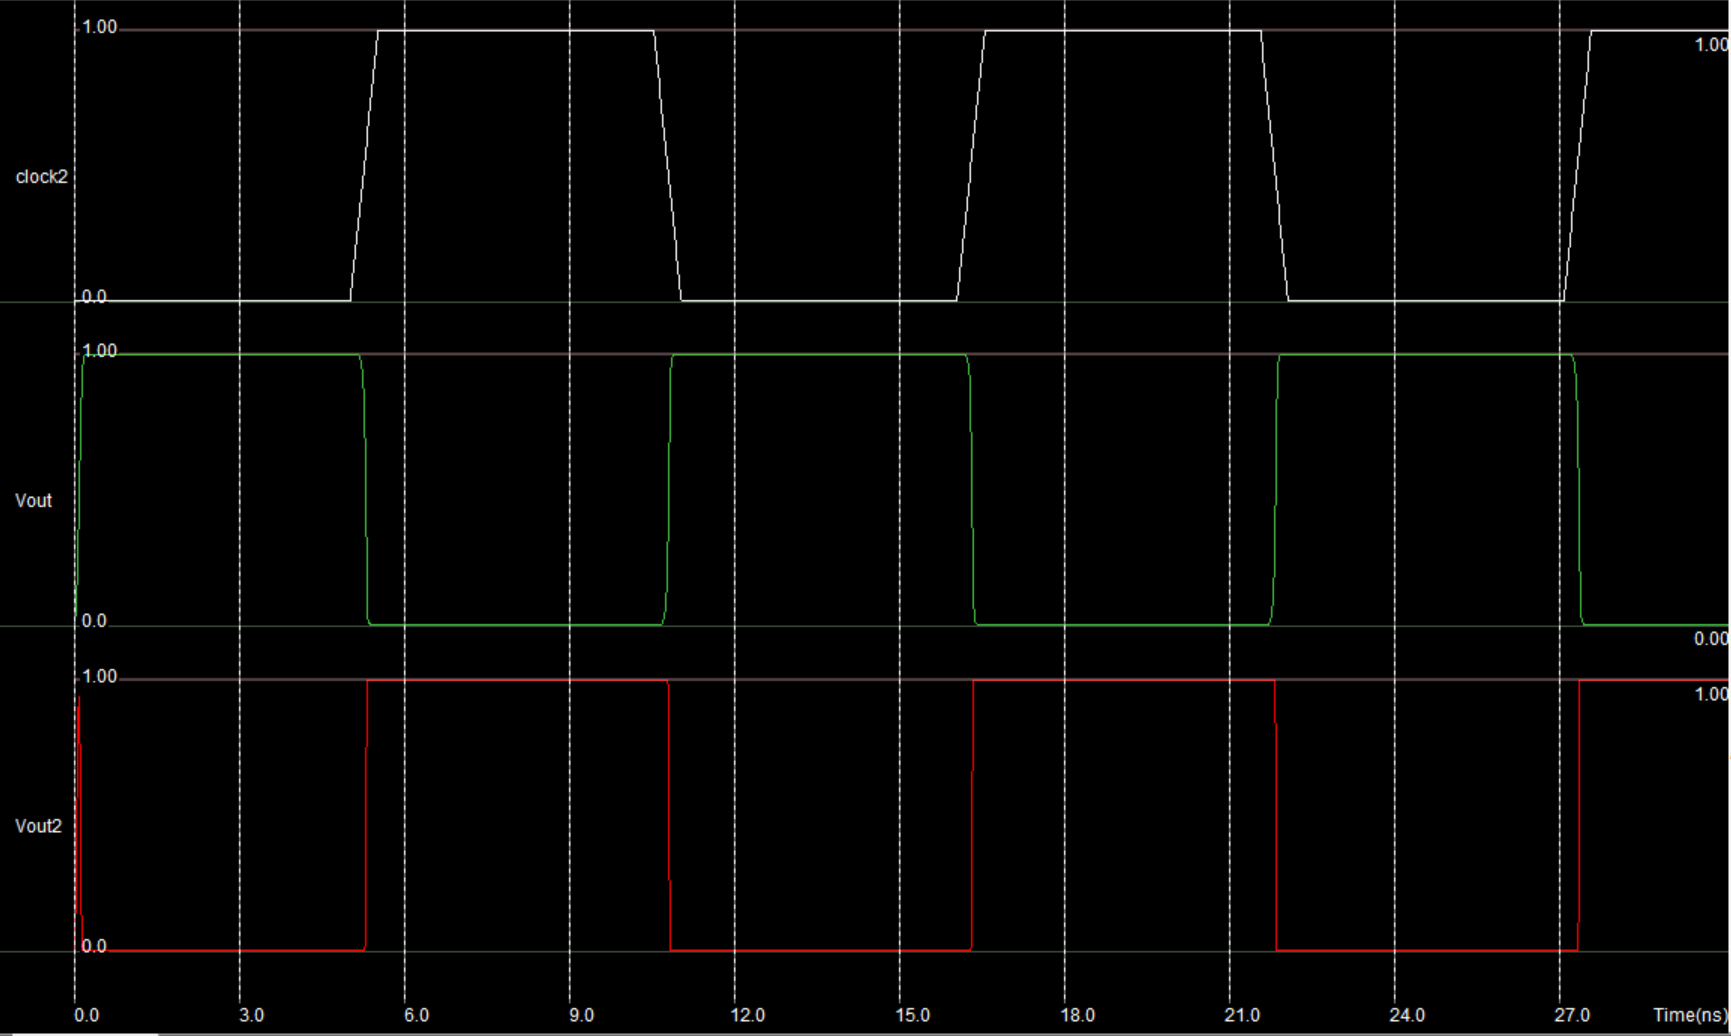
\includegraphics[scale=0.50]{./images/cascaded_inverter_transient_06nmos15pmos.PNG}
	\caption{Cascaded Inverter Transient - 0.6\si{\micro\meter} Width for NMOS, 1.5 \si{\micro\meter} Width for PMOS}
	\label{fig:cascaded_inverter_transient_06nmos15pmos}
\end{figure}

\FloatBarrier

The widths of the NMOS and PMOS are then increased to 1.2\si{\micro\meter} and 3.0\si{\micro\meter} respectively.

\FloatBarrier

\begin{figure}[h!]
	\centering
	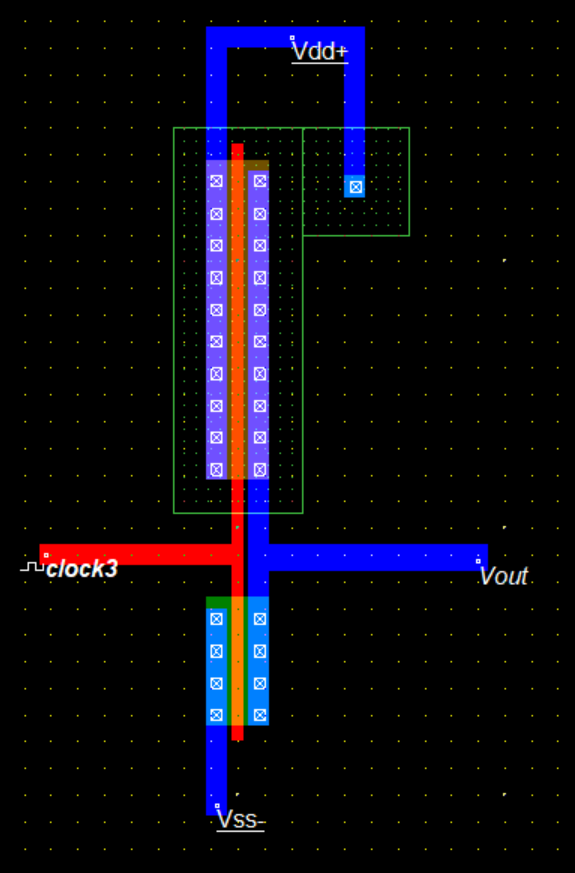
\includegraphics[scale=0.75]{./images/inverter_12nmos30pmos.PNG}
	\caption{Layout of CMOS Inverter - 1.2\si{\micro\meter} Width for NMOS, 3.0 \si{\micro\meter} Width for PMOS}
	\label{fig:inverter_12nmos30pmos}
\end{figure}

\FloatBarrier

\FloatBarrier

\begin{figure}[h!]
	\centering
	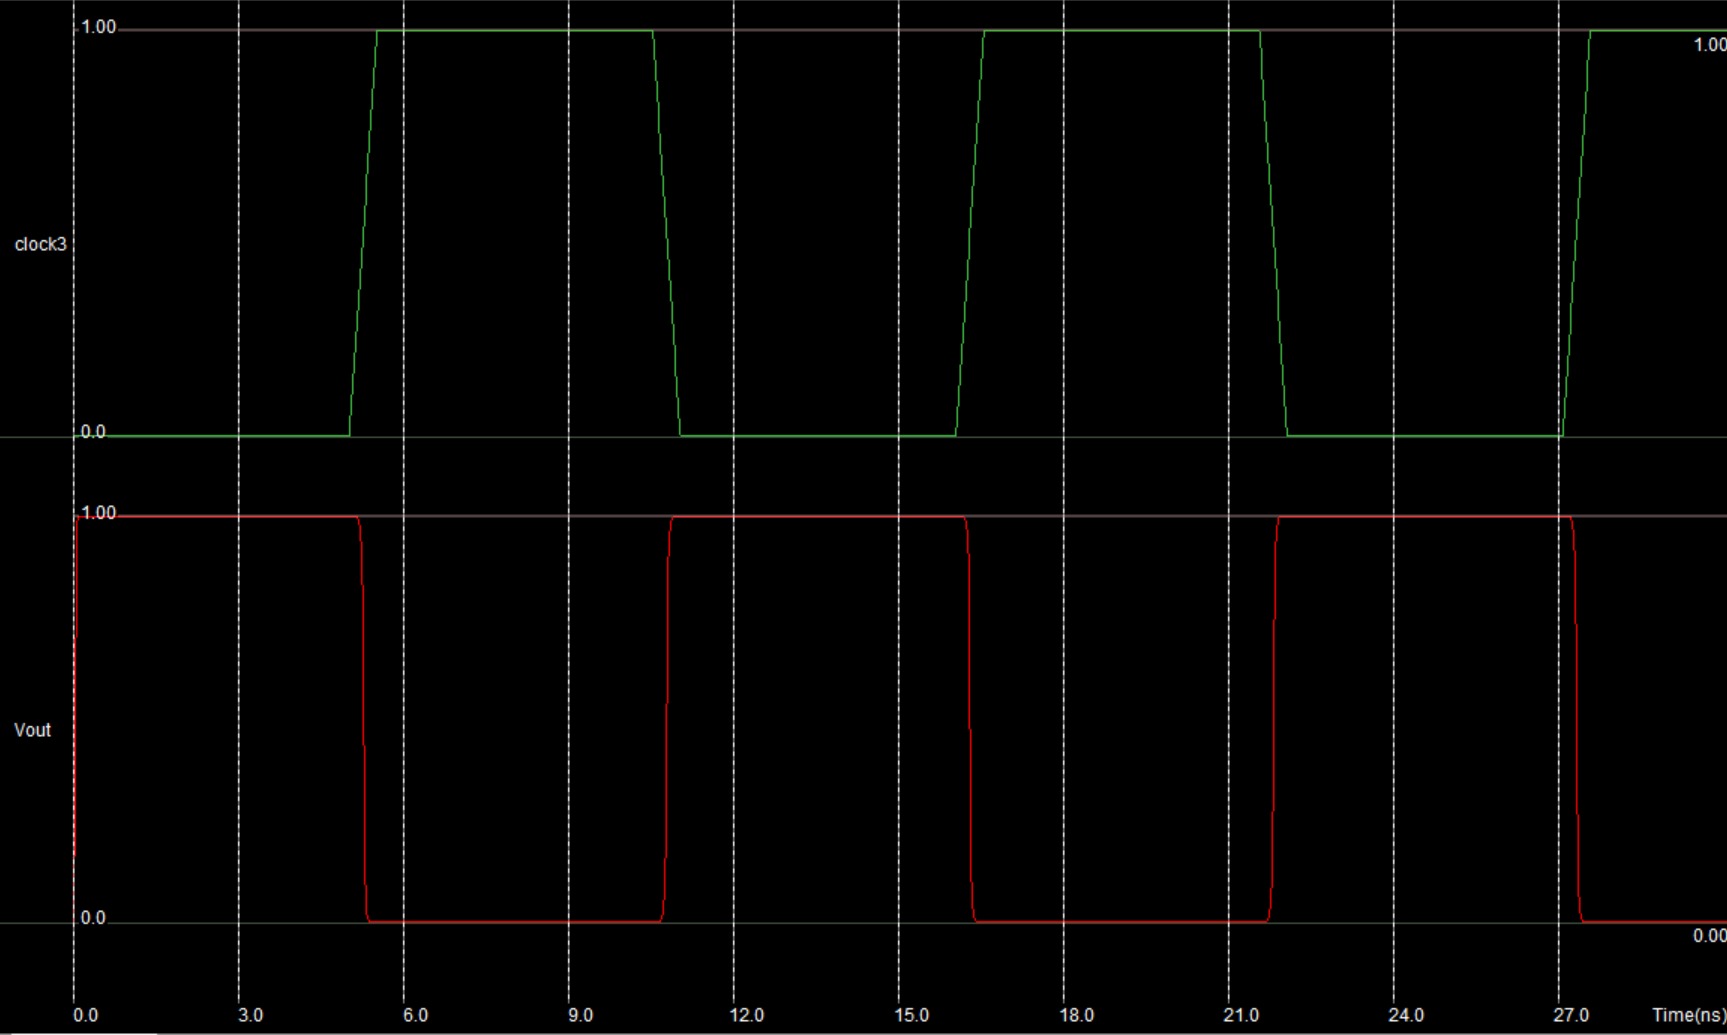
\includegraphics[scale=0.50]{./images/inverter_transient_12nmos_30pmos.PNG}
	\caption{CMOS Inverter Layout Transient Response - 1.2\si{\micro\meter} Width for NMOS, 3.0 \si{\micro\meter} Width for PMOS}
	\label{fig:inverter_transient_12nmos_30pmos}
\end{figure}

\FloatBarrier

\FloatBarrier

\begin{figure}[h!]
	\centering
	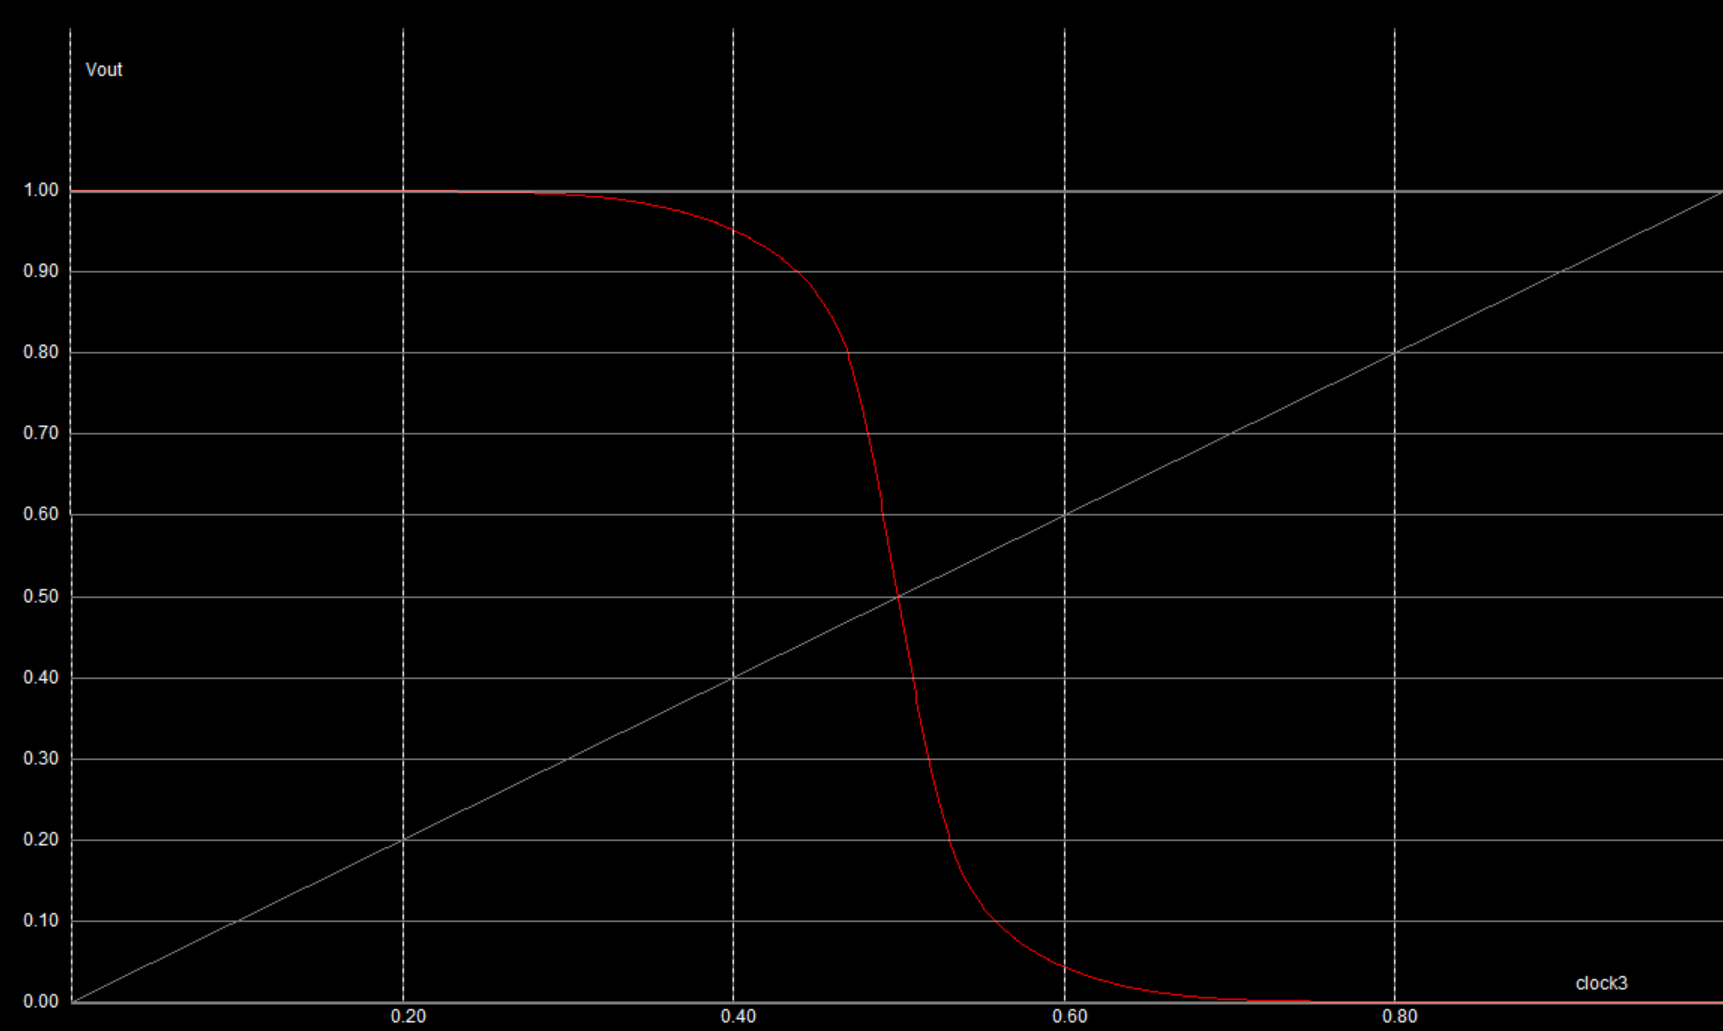
\includegraphics[scale=0.50]{./images/inverter_vtc_12nmos_30pmos.PNG}
	\caption{CMOS Inverter Layout Voltage Transfer Characteristic (VTC) - 1.2\si{\micro\meter} Width for NMOS, 3.0 \si{\micro\meter} Width for PMOS}
	\label{fig:inverter_vtc_12nmos_30pmos}
\end{figure}

\FloatBarrier

\FloatBarrier

\begin{figure}[h!]
	\centering
	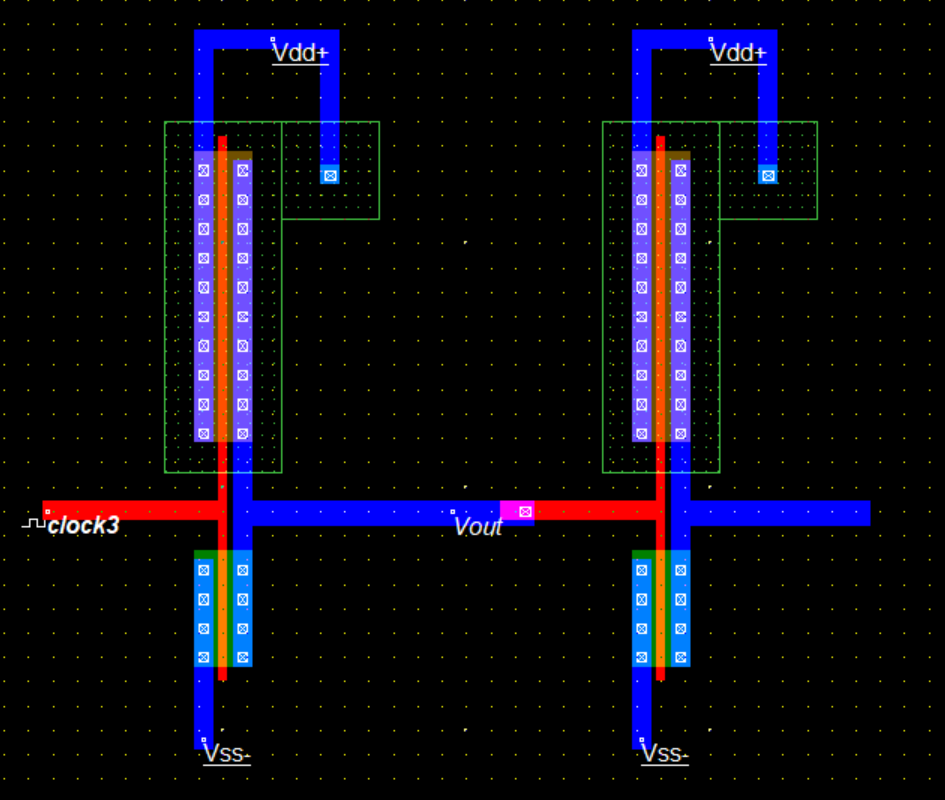
\includegraphics[scale=0.75]{./images/cascaded_inverter_12nmos_30pmos.PNG}
	\caption{Cascaded Inverter Layout - 1.2\si{\micro\meter} Width for NMOS, 3.0 \si{\micro\meter} Width for PMOS}
	\label{fig:cascaded_inverter_12nmos30pmos}
\end{figure}

\FloatBarrier

\FloatBarrier

\begin{figure}[h!]
	\centering
	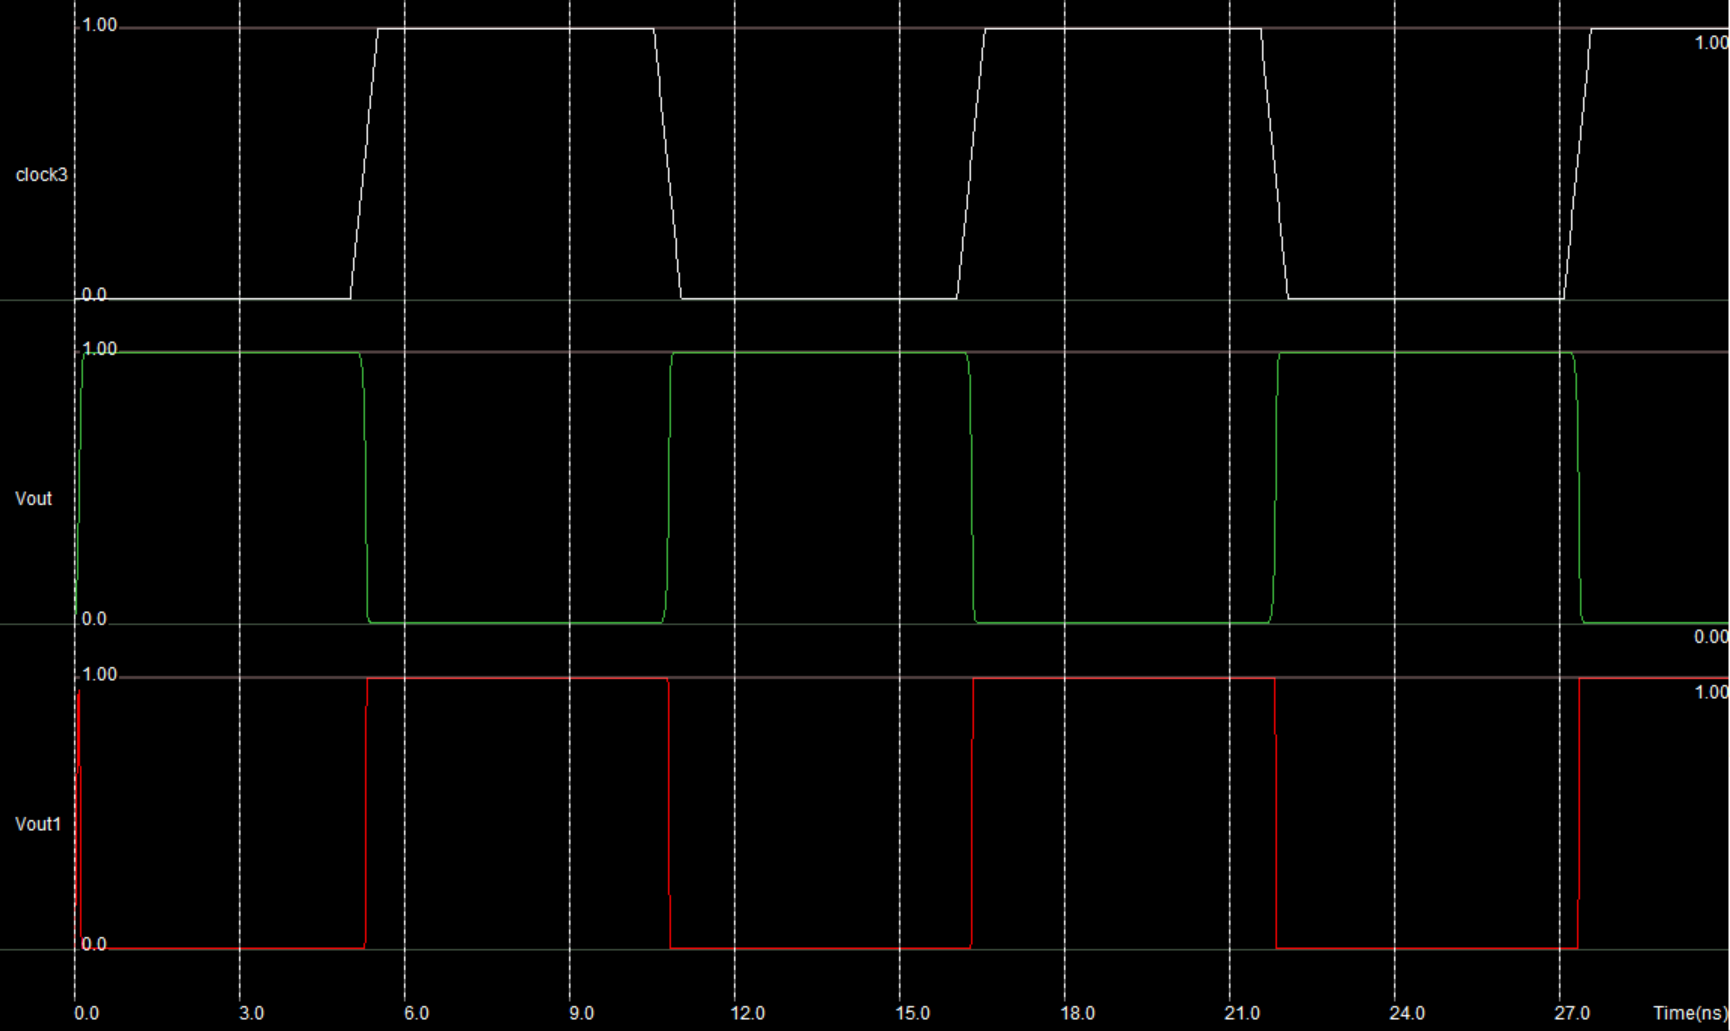
\includegraphics[scale=0.50]{./images/cascaded_inverter_transient_12nmos_30pmos.PNG}
	\caption{Cascaded Inverter Transient - 1.2\si{\micro\meter} Width for NMOS, 3.0 \si{\micro\meter} Width for PMOS}
	\label{fig:cascaded_inverter_transient_12nmos30pmos}
\end{figure}

\FloatBarrier

The propagation delays, $t_{PHL}$, $t_{PLH}$, and $t_{P} = \frac{ t_{PHL} + t_{PLH} }{2}$, for the single inverter simulations are reported in table (\ref{tab:single_inverter_delay}).
$t_{P}$ is calculated from $t_{PHL}$ and $t_{PLH}$.
$t_{PHL}$ and $t_{PLH}$ are taken directly from the simulation itself.

\FloatBarrier

\begin{table}[h!]
	\centering
	\caption{Single Inverter Delays}
	\label{tab:single_inverter_delay}
	\csvautotabular{./tables/single_inverter_delay.csv}
\end{table}

\FloatBarrier

The delays for the first inverter in the cascaded inverter simulation are reported in table (\ref{tab:double_inverter_delays}).

\FloatBarrier

\begin{table}[h!]
	\centering
	\caption{Cascaded Inverter Delays - First Inverter}
	\label{tab:double_inverter_delays}
	\csvautotabular{./tables/double_inverter_delays.csv}
\end{table}

\FloatBarrier

The second inverter delays are taken with respect to the input of the first inverter.
It is quite difficult to ascertain accurate delays for the second inverter relative to the first inverter's output from the simulation tool.
$t_{PLH}$ for the first simulation reported by the tool seems dubious due to the fact that it is only a mere $2$\si{\pico\second}, but the results demonstrate general trends.
The values are reported in table (\ref{tab:double_inverter_delays_2}).

\FloatBarrier

\begin{table}[h!]
	\centering
	\caption{Cascaded Inverter Delays - Second Inverter}
	\label{tab:double_inverter_delays_2}
	\csvautotabular{./tables/double_inverter_delays_2.csv}
\end{table}

\FloatBarrier

For the single inverter simulation, the delay drops considerably as the widths of the transistors are increased. The results taper off as widths are increased. There are various inherent delays in components due to parasitic inductances and capacitances of the wires and physical limitations on speed. So, a certain amount of delay must always exist. Increasing widths should then become less effective as the widths become very large.
By "delay", the amount of time it would take to charge a load capacitance connected at the output, such as the MOS capacitors of the next stage of transistors as well as parasitic capacitances, is implied. So, if the transistors are able to drive more current to the load capacitance, then the load charges more quickly, and the delay drops. So, the reason the delay drops is because increasing the width of the transistor allows more charge per unit time to flow, causing larger currents to more quickly charge a load.
For the cascaded inverters, the first inverter's delay decreases, but not as much as it does in the single inverter delay measurements. When only one inverter is present, the voltage can quickly form at the output port after the gate voltage is set. It is limited only by some of the material properties of the transistors in the inverter. However, when an inverter is connected at the load, not only must the output current be generated, which takes time due to the formation of the channel, but the capacitances of the MOSFETs in the next inverter stage and the parasitic capacitances must be charged with that current. So, it takes a little bit longer for the voltage to form, which is why the delay is longer.
The delay of the second inverter in the cascade from the input to the first inverter is generally not much longer, maybe by only a few picoseconds, than the delay of the first inverter. Once the voltage has formed at the input of the second inverter, it reduces to the case with a single inverter. So, by the same reasons as above, the voltage at the output should form more quickly than if it were a loaded inverter in an intermediary stage of two cascaded inverters. \\

When the PMOS inverter's width is made so that its transconductance parameter is balanced with the NMOS, the VTC shifts to the right. When the input to the inverter is low, the PMOS is enabled. PMOS transistors have holes as their charge carrier, and thus their mobility is lower than that of electrons in the NMOS. So, in the $0.6$\si{\micro\meter} for both NMOS and PMOS test, both have the same dimensions, and the NMOS's transconductance parameter is dominant. If the PMOS's transcondunctance parameter is relatively smaller, then the current it produces is relatively smaller. If the voltage is increased, the NMOS transistor begins to turn on and enter saturation. So, a current starts to flow through both transistors. However, the PMOS cannot support as large of a current. If the PMOS and NMOS are seen as resistors in this state, the PMOS would have a much larger equivalent resistance, and thus the NMOS would take up a smaller voltage drop, meaning $V_{out}$ is smaller. So, $V_{out}$ drops more quickly as $V_{in}$ is increased because the PMOS quickly consumes a much larger voltage drop.
When the transistor sizes are changed from $0.6$\si{\micro\meter} for the PMOS and NMOS to $0.6$\si{\micro\meter} for the NMOS and $1.5$\si{\micro\meter} for the PMOS, the transistors are now more balanced, meaning their transconductance parameters are closer in magnitude. If this is the case, the currents that each can supply are comparable. If the voltage divider analogy is revisited, the "resistances" -- in a sense -- of each transistor are closer in magnitude than in the previous case. So, as $V_{in}$ is increased, the NMOS transistor can sustain a higher voltage drop for longer than when the PMOS's "equivalent resistance" far outweighed the NMOS's. So, the VTC shifts to the right when the transistors become balanced as opposed to the previous unbalanced case. It should be noted that modeling either of these components as a resistor is not entirely accurate since their voltages are not linearly related to their currents, but the voltage divider analogy can be used to understand why the VTC shifts when the transistors move from NMOS having the dominant parameter to balanced parameters.
